\documentclass[a4paper]{article}
\usepackage{vntex}
%\usepackage[english,vietnam]{babel}
%\usepackage[utf8]{inputenc}

%\usepackage[utf8]{inputenc}
%\usepackage[francais]{babel}
\usepackage{a4wide,amssymb,epsfig,latexsym,multicol,array,hhline,fancyhdr}
\usepackage{booktabs}
\usepackage{amsmath}
\usepackage{lastpage}
\usepackage[lined,boxed,commentsnumbered]{algorithm2e}
\usepackage{enumerate}
\usepackage{color}
\usepackage{graphicx}							% Standard graphics package
\usepackage{array}
\usepackage{tabularx, caption}
\usepackage{multirow}
\usepackage[framemethod=tikz]{mdframed}% For highlighting paragraph backgrounds
\usepackage{multicol}
\usepackage{rotating}
\usepackage{graphics}
\usepackage{geometry}
\usepackage{setspace}
\usepackage{epsfig}
\usepackage{tikz}
\usepackage{listings}
\usetikzlibrary{arrows,snakes,backgrounds}
\usepackage{hyperref}
\usepackage{parskip}
\hypersetup{urlcolor=blue,linkcolor=black,citecolor=black,colorlinks=true} 
%\usepackage{pstcol} 								% PSTricks with the standard color package

\newtheorem{theorem}{{\bf Định lý}}
\newtheorem{property}{{\bf Tính chất}}
\newtheorem{proposition}{{\bf Mệnh đề}}
\newtheorem{corollary}[proposition]{{\bf Hệ quả}}
\newtheorem{lemma}[proposition]{{\bf Bổ đề}}

\everymath{\color{blue}}
%\usepackage{fancyhdr}
\setlength{\headheight}{40pt}
\pagestyle{fancy}
\fancyhead{} % clear all header fields
\fancyhead[L]{
 \begin{tabular}{rl}
    \begin{picture}(25,15)(0,0)
    \put(0,-8){
\includegraphics[width=8mm, height=8mm]{logoITSGUsmall.png}}
    %\put(0,-8){\epsfig{width=10mm,figure=hcmut.eps}}
   \end{picture}&
	%\includegraphics[width=8mm, height=8mm]{hcmut.png} & %
	\begin{tabular}{l}
		\textbf{\bf \ttfamily Trường Đại học Sài Gòn}\\
		\textbf{\bf \ttfamily Khoa Công Nghệ Thông Tin}
	\end{tabular} 	
 \end{tabular}
}
\fancyhead[R]{
	\begin{tabular}{l}
		\tiny \bf \\
		\tiny \bf 
	\end{tabular}  }
\fancyfoot{} % clear all footer fields
\fancyfoot[L]{\scriptsize \ttfamily Bài tập lớn môn Phát triển phần mềm mã nguồn mở - Niên khóa 2023-2024}
\fancyfoot[R]{\scriptsize \ttfamily Trang {\thepage}/\pageref{LastPage}}
\renewcommand{\headrulewidth}{0.3pt}
\renewcommand{\footrulewidth}{0.3pt}


%%%
\setcounter{secnumdepth}{4}
\setcounter{tocdepth}{3}
\makeatletter
\newcounter {subsubsubsection}[subsubsection]
\renewcommand\thesubsubsubsection{\thesubsubsection .\@alph\c@subsubsubsection}
\newcommand\subsubsubsection{\@startsection{subsubsubsection}{4}{\z@}%
                                     {-3.25ex\@plus -1ex \@minus -.2ex}%
                                     {1.5ex \@plus .2ex}%
                                     {\normalfont\normalsize\bfseries}}
\newcommand*\l@subsubsubsection{\@dottedtocline{3}{10.0em}{4.1em}}
\newcommand*{\subsubsubsectionmark}[1]{}
\makeatother

\definecolor{dkgreen}{rgb}{0,0.6,0}
\definecolor{gray}{rgb}{0.5,0.5,0.5}
\definecolor{mauve}{rgb}{0.58,0,0.82}

\lstset{frame=tb,
	language=Matlab,
	aboveskip=3mm,
	belowskip=3mm,
	showstringspaces=false,
	columns=flexible,
	basicstyle={\small\ttfamily},
	numbers=none,
	numberstyle=\tiny\color{gray},
	keywordstyle=\color{blue},
	commentstyle=\color{dkgreen},
	stringstyle=\color{mauve},
	breaklines=true,
	breakatwhitespace=true,
	tabsize=3,
	numbers=left,
	stepnumber=1,
	numbersep=1pt,    
	firstnumber=1,
	numberfirstline=true
}

\begin{document}

\begin{titlepage}
\begin{center}
TRƯỜNG ĐẠI HỌC SÀI GÒN \\
KHOA CÔNG NGHỆ THÔNG TIN
\end{center}
\vspace{1cm}

\begin{figure}[h!]
\begin{center}

\includegraphics[width=3cm]{logoITSGU.png}
\end{center}
\end{figure}

\vspace{1cm}


\begin{center}
\begin{tabular}{c}
	\multicolumn{1}{l}{\textbf{{\Large PHÁT TRIỂN PHẦN MỀM MÃ NGUỒN MỞ}}}\\
	~~\\
	\hline
	\\
	\multicolumn{1}{l}{\textbf{{\Large Đề tài: }}}\\
	\\
	
	\textbf{{\Huge Trò chơi bắn xe tăng}}\\
	\\
	\hline
\end{tabular}
\end{center}

\vspace{3cm}

\begin{table}[h]
\begin{tabular}{rrl}
\hspace{5 cm} & Giảng viên hướng dẫn: &Từ Lãng Phiêu\\
& Nhóm thực hiện: & Nhóm 18\\
& Sinh viên thực hiện: & 3120410620 – Lê Thanh Vũ\\
& & 3120410426 – Nguyễn Thanh Quang \\
& & 3120410635 – Đặng Huỳnh Như Y \\
% & & SV3 - MSSV \\
% & & SV4 - MSSV\\
\end{tabular}
\vspace{1.5 cm}
\end{table}

\begin{center}

{\footnotesize TP. HỒ CHÍ MINH, THÁNG 4/2024}
\end{center}
\end{titlepage}


\thispagestyle{empty}

\newpage
\begin{center}
DANH SÁCH THÀNH VIÊN NHÓM 18 \\
\end{center}
\vspace{1cm}

% \begin{center}

% \begin{tabular}{ |c|c|c| }
%   \hline
%   MSSV & Họ tên & Gmail \\ \hline
%   3120410620 & Lê Thanh Vũ & thanhvu270202@gmail.com \\ \hline
%   3120410426 & Nguyễn Thanh Quang & Quang.kasumi@gmail.com \\ \hline
%   3120410635 & Đặng Huỳnh Như Y & nhuy.danghuynh2002@gmail.com \\ 
%   \hline
% \end{tabular} 
% \end{center}

\begin{center}
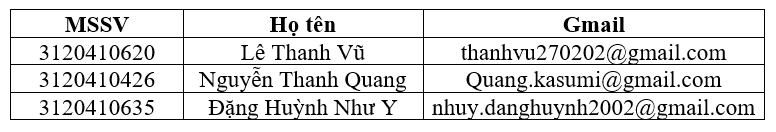
\includegraphics[width=6in,height=1in]{image1_1.png}
\end{center}

\newpage
\tableofcontents
\newpage

%%%%%%%%%%%%%%%%%%%%%%%%%%%%%%%%%


%%%%%%%%%%%%%%%%%%%%%%%%%%%%%%%%%
\section{TỔNG QUAN GIAO DIỆN}
\subsection{Các thành phần trên giao diện}
Giao diện được thiết kế bằng PyQT5 bao gồm một cửa sổ hiển thị hình ảnh
giới thiệu chương trình, với 3 nút để chuyển đổi giữa các chế độ và nút
thoát để đóng giao diện, cũng như có phần mô tả và biểu tượng của chương
trình. \vspace{1em} \\
Phương thức \textbf{`\_\_init\_\_}` được sử dụng để khởi tạo đối tượng
của một lớp. Nó gọi phương thức khởi tạo của lớp cha, thiết lập các
thuộc tính như `\textbf{title}`, `\textbf{left}`, `\textbf{top}`,
`\textbf{width}`, `\textbf{height}`, và gọi phương thức
`\textbf{initUI}` để khởi tạo giao diện người dùng. \vspace{1em}\\
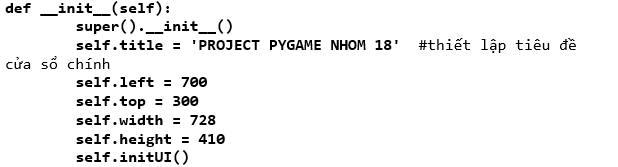
\includegraphics[width=5.5in,height=1.5in]{image1_2.png}

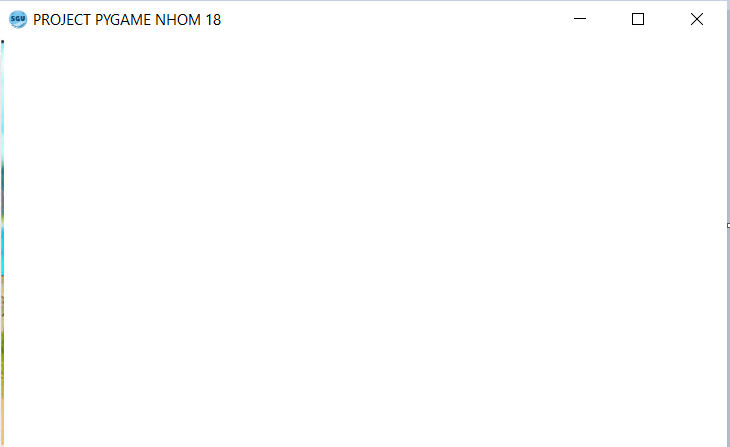
\includegraphics[width=6.3in,height=3.85833in]{image2.png}\\
	
\subsection{Tạo đối tượng button và xử lí sự kiện}
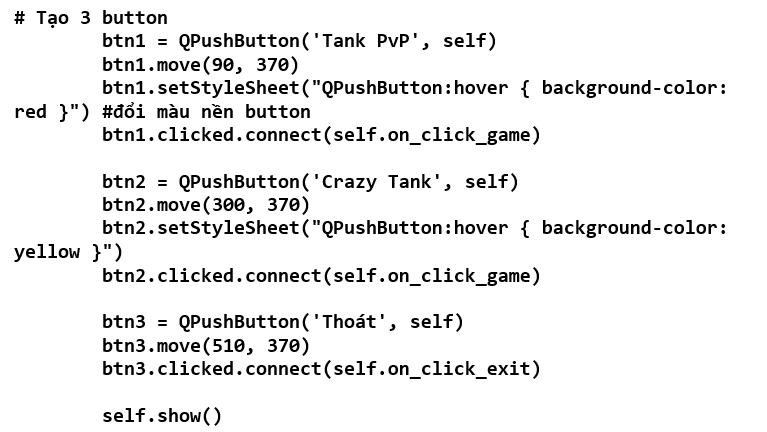
\includegraphics[width=6in,height=3.7in]{image1_3.png}

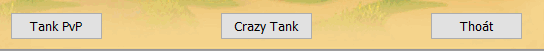
\includegraphics[width=5.66528in,height=0.53194in]{image3.png}\vspace{1em}\\
Ta tạo nút nhấn có tên \textbf{``Tank PvP''} tương ứng với chế độ cùng tên và set vị trí chúng cho phù hợp trên trục tọa độ Oxy \textbf{(90,370)}, và tạo hàm xử lí để xử lí sự kiện này, từ đó ta thực hiện các chế độ khác tương tự. Để
thu hút người chơi thì nhóm đã tạo thêm hiệu ứng cho các butto khi click
vào.\vspace{1em}\\
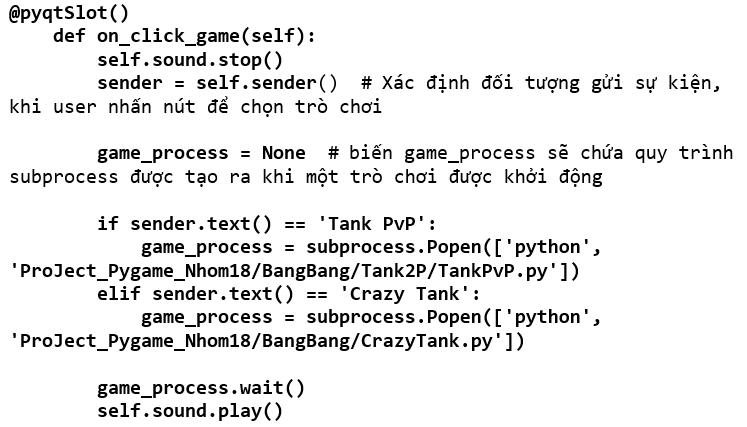
\includegraphics[width=6in,height=3in]{image3_2.png}\vspace{1em}\\
Một phương thức được gắn với một slot PyQt, được kích hoạt khi một sự
kiện nhất định xảy ra (dừng nhạc nền, khởi động game mà người dùng chọn
từ giao diện, khi người dùng thoát game thì phát lại nhạc nền).\\
Khi ta nhấn nút thoát, chương trình sẽ gọi đến hàm
\textbf{on\_click\_exit()} sẽ gọi đến phương thức thoát chương trình.\vspace{1em}\\
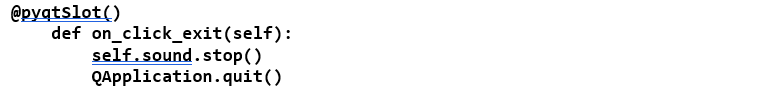
\includegraphics[width=5in,height=0.7in]{image3_3.png}\vspace{1em}\\
\textbf{Giao diện chương trình sau khi hoàn chỉnh:}\vspace{1em}\\
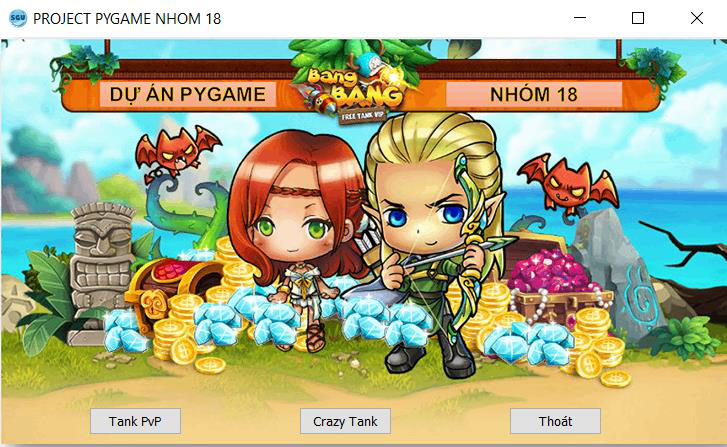
\includegraphics[width=5.25in,height=3.22778in]{image4.png}
%%%%%%%%%%%%%%%%%%%%%%%%%%%%%%%%%

%%%%%%%%%%%%%%%%%%%%%%%%%%%%%%%%%
\newpage
\section{MODE GAME VƯỢT MƯA THIÊN THẠCH}
\subsection{Giới thiệu}\vspace{1em}
Chào mừng đến với game "Crazy Tank":
Bạn đã sẵn sàng tham gia vào một cuộc phiêu lưu ngoài vũ trụ đầy kịch
tính và hấp dẫn chưa? Trong trò chơi này, bạn sẽ nhập vai là một chiến
binh tinh nhuệ điều khiển chiếc tank mạnh mẽ để chiến đấu chống lại các
cơn mưa thiên thạch nguy hiểm.

Nhiệm vụ của bạn là di chuyển tank một cách linh hoạt, né tránh tất cả
các thiên thạch trên đường đi để bảo vệ không gian ngoài vũ trụ. Sử dụng
kỹ năng và phản xạ nhanh nhạy để vượt qua những thách thức khó khăn và
giành chiến thắng.

Để tối ưu hóa trò chơi và làm cho cách chơi trở nên dễ dàng hơn, phù hợp
với mọi độ tuổi và thiết bị, nhóm em sử dụng cơ chế điều khiển thông qua
chuột hoặc cảm ứng trên các điện thoại có màn hình cảm ứng với chỉ một
thao tác duy nhất để điều khiển. Điều này giúp người chơi dễ dàng tương
tác với trò chơi một cách tự nhiên và thuận tiện, mang lại trải nxuấtệm
chơi game tốt hơn và thú vị hơn.
chơi game tốt hơn và thú vị hơn.

\subsection{Hướng dẫn cách chơi}

\textbf{Bước 1:} Người chơi chỉ cần thao tác điều khiển xe tăng bằng
chuột hoặc touchpad trên laptop để di chuyển xe theo hướng mong muốn,
tạo cảm giác dễ dàng và linh hoạt khi chơi.

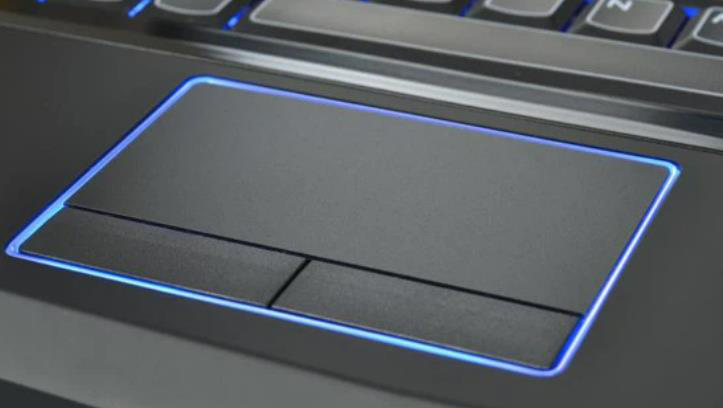
\includegraphics[width=3.60417in,height=1.95in]{image5.png}

\textbf{Bước 2:} Trong trò chơi "Crazy Tank", người chơi cần nhặt hộp
quà để tích điểm, né tránh thiên thạch để sống sót và tích điểm nhanh
nhất. Điều này yêu cầu phản xạ nhanh nhạy và kỹ năng điều khiển xe tăng
để đạt điểm số cao nhất.

.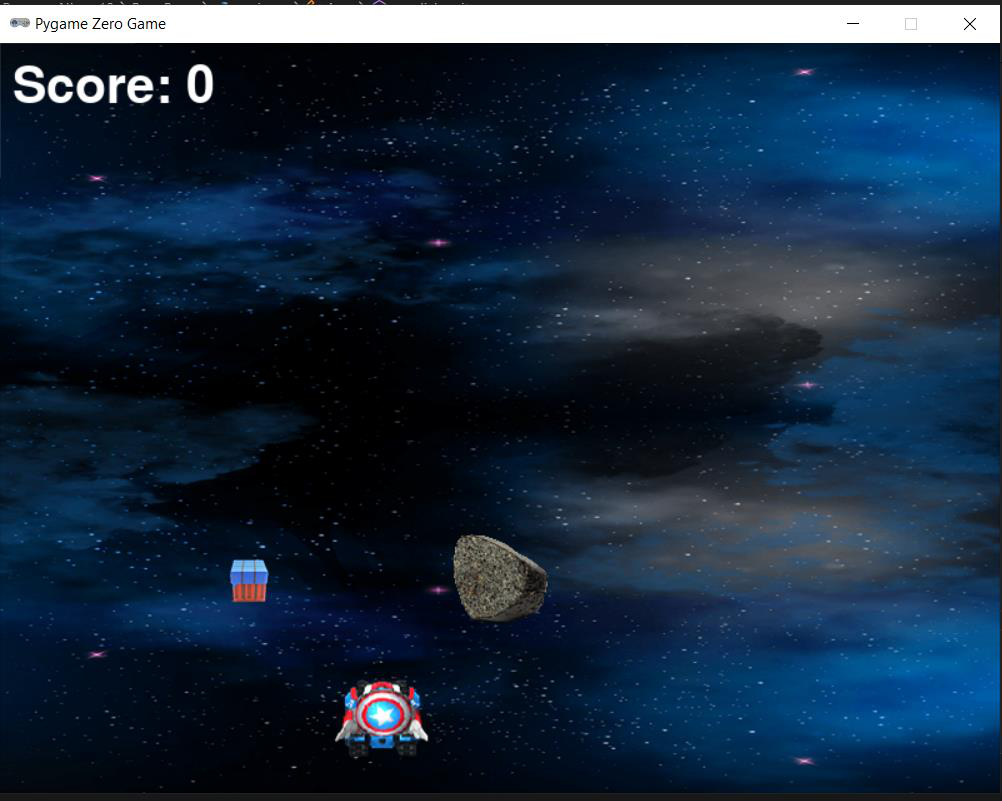
\includegraphics[width=6.15555in,height=3.90556in]{image6.png}

\textbf{Lưu ý:} Khi người chơi thu thập đủ nhiều hộp quà thì tốc độ của
trò chơi sẽ tăng lên càng lúc càng nhanh để tăng thêm độ khó cho trò chơi, bên cạnh đó càng ngày theo độ khó của trò chơi âm nhạc sẽ sôi động hơn và nhịp nhanh hơn.
\newpage
\subsection{Ý tưởng}

Trong trò chơi, ta có ba đối tượng chính:

- Xe tăng: Điều khiển bởi người chơi, tự động tiến lên và không thể dừng
lại. - Hộp quà: Biểu diễn bằng hộp quà có hình dạng đặc trưng, người
chơi cần nhặt để tích điểm.

- Thiên thạch : Được biểu diễn bằng các khối thiên thạch, nguy hiểm và
người chơi cần tránh để tránh bị tiêu diệt.

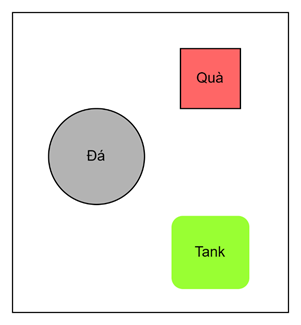
\includegraphics[width=2.27083in,height=2.45139in]{image7.png}

Trong trò chơi, người chơi điều khiển xe tăng để nhặt hộp quà và tránh
thiên thạch để tích điểm và duy trì sự sống. Hộp quà và thiên thạch xuất
hiện ngẫu nhiên trên bản đồ, tạo sự bất ngờ và thách thức, tăng cường
hứng thú và cảm giác thử thách khi chơi.

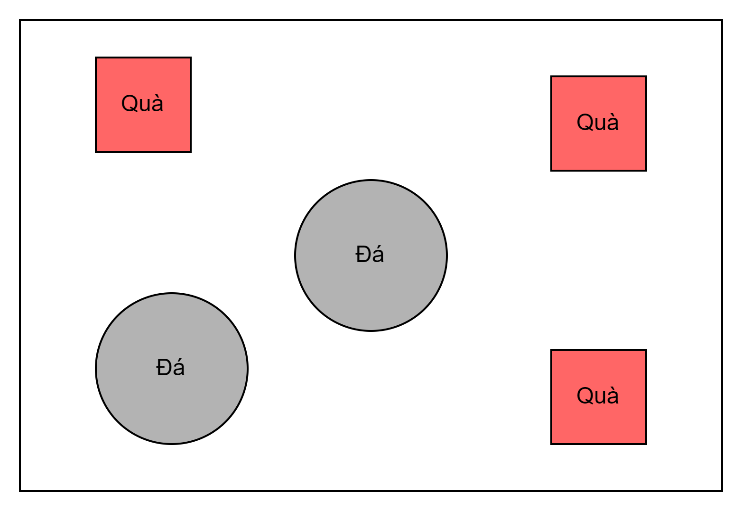
\includegraphics[width=3.36806in,height=2.32222in]{image8.png}

Để tạo cảm giác xe tăng di chuyển tốc độ cao, hộp quà và thiên thạch rơi
xuống từ trên xuống, giúp người chơi cảm thấy như đang phải phản xạ
nhanh để nhặt hộp quà và tránh thiên thạch. Việc này tạo cảm giác động
đất và thú vị khi chơi.

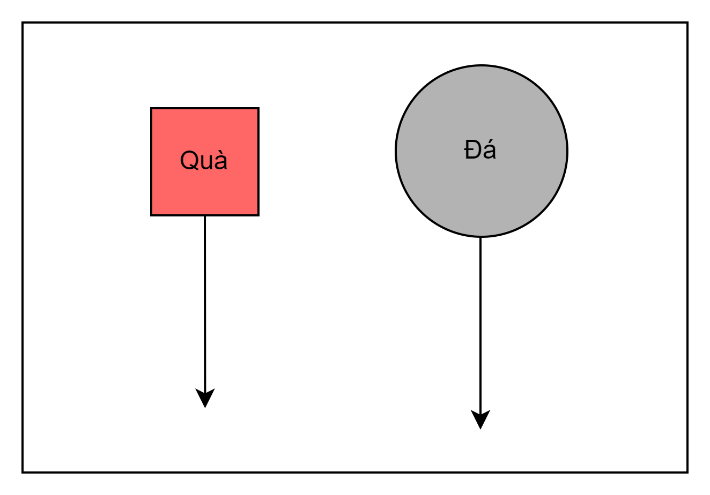
\includegraphics[width=3.22639in,height=2.25in]{image9.png}

Để hướng người chơi né thiên thạch và nhặt hộp quà, áp dụng các chiến
lược như đặt hộp quà gần thiên thạch, tăng tốc độ rơi của hộp quà, và
đặt hộp quà ở vị trí chiến lược. Những chiến lược này tạo thách thức và
khuyến khích người chơi kết hợp kỹ năng để đạt điểm số cao.

\subsection{Mô hình chương trình}
Cơ chế quá trình hoạt động

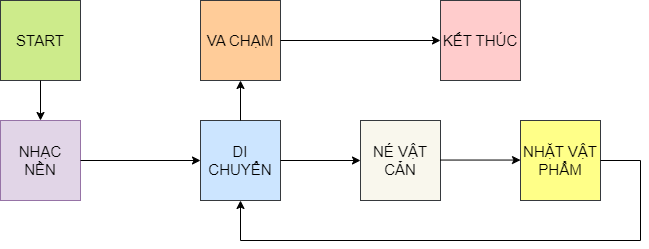
\includegraphics[width=4.79722in,height=1.84583in]{image11.png}
\newpage
\subsection{Quy trình thực hiện}
\subsubsection{Thư viện cần dùng}
\textbf{import pgzrun, random}\\
\textbf{from random import randint}

Trong trò chơi sử dụng thư viện \textbf{pgzero} của \textbf{Pygame}, việc sử dụng thư viện \textbf{random} để xuất hiện các vật thể như hộp quà và thiên thạch một cách ngẫu nhiên giúp tạo ra sự đa dạng và hấp dẫn cho trò chơi. Bằng
cách này, người chơi sẽ không gặp phải sự lặp lại và nhàm chán trong
trải nghiệm chơi game của họ. Đồng thời, việc sử dụng \textbf{pgzero} giúp phát
triển trò chơi một cách dễ dàng và hiệu quả cho các trò chơi có quy mô
nhỏ và đơn giản.
\subsubsection{Cài đặt một số biến cơ bản}
\textbf{WIDTH, HEIGHT = 800, 600}\\
\textbf{WHITE, VIOLET = (255,255,255), (255,0,255)}\\ 
\textbf{diem = 0}\\
\textbf{ket\_thuc = False}\\
\textbf{background.draw()}

Thiết lập kích thước cửa sổ, màu sắc và tính điểm khi nhặt hộp quà là
những điểm quan trọng trong trò chơi, tạo trải nxuấtệm hấp dẫn cho người
chơi.
\subsubsection{Định dạng hình ảnh và vị trí}
\textbf{\# Định dạng hình nền}\\
\textbf{background = Actor("nengame")}

\textbf{\# Định dạng tank, hộp quà, thiên thạch tank =
Actor(\textquotesingle captain\textquotesingle)}\\
\textbf{tank.x, tank.y = 100, 550}\\
\textbf{item = Actor(\textquotesingle hopqua\textquotesingle)}\\
\textbf{item.x, item.y = 200, 0}\\
\textbf{rock = Actor(\textquotesingle thienthach\textquotesingle)}\\
\textbf{rock.x, rock.y = 400, 0}

Ta sẽ gán đường dẫn của các hình ảnh cho các biến để dễ thao tác với
chúng, vị trí của chúng được xác định dựa trên trục tọa độ Oxy.

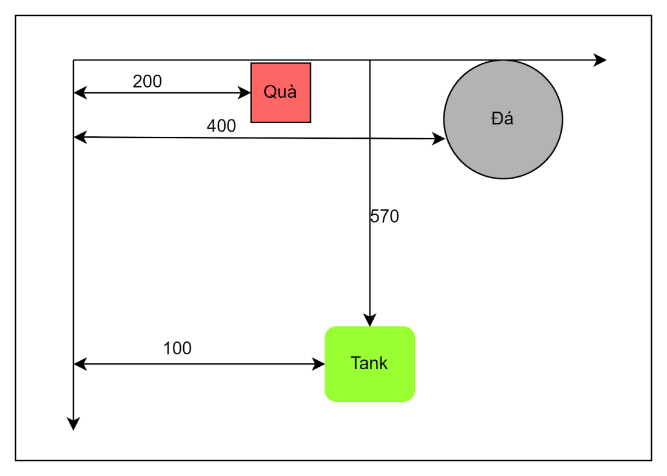
\includegraphics[width=2.99583in,height=2.14306in]{image12.png}

Trong trò chơi, vị trí ban đầu tạm thời của các đối tượng được thiết lập
như sau: \\
- Xe tăng: vị trí ban đầu tại \textbf{x = 100}, \textbf{y = 550}. Xe tăng sẽ được điều khiển bởi chuột khi người chơi chơi.

- Hộp quà: vị trí ban đầu tại \textbf{x = 200}, \textbf{y = 0}. Hộp quà sẽ xuất hiện ngẫu nhiên trong trò chơi để người chơi nhặt.

- Thiên thạch: vị trí ban đầu tại \textbf{x = 400}, \textbf{y = 0}. Thiên thạch cũng sẽ xuất hiện ngẫu nhiên trong trò chơi, tạo thêm thách thức cho người chơi.
\subsubsection{Cơ chế điều khiển xe tăng}
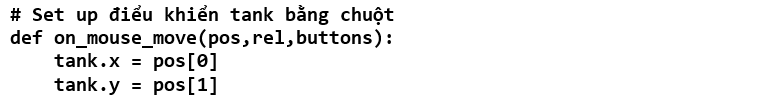
\includegraphics[width=5.5in,height=0.6in]{image12_2.png}

Trong trò chơi, việc điều khiển xe tăng bằng chuột giúp người chơi linh
hoạt di chuyển xe tăng theo vị trí chuột trên màn hình. Các tham số như
`\textbf{pos}`, `\textbf{rel}`, và `\textbf{buttons}` được sử dụng để
xác định vị trí và trạng thái của chuột trong quá trình điều khiển.

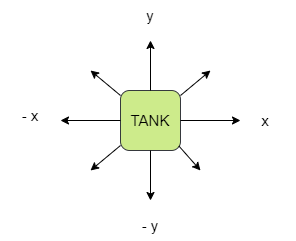
\includegraphics[width=2.58333in,height=2.10139in]{image13.png}
\subsubsection{Tăng tốc độ của trò chơi}
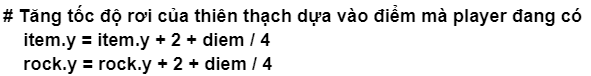
\includegraphics[width=4.5in,height=0.5in]{image13_1.png}

Trong trò chơi, tốc độ rơi của hộp quà và thiên thạch tăng dần theo điểm
số của người chơi. Việc này tạo ra sự thách thức gia tăng khi người chơi
cố gắng đạt điểm số cao hơn để đối phó với tốc độ tăng của trò chơi.
\subsubsection{Xử lí khi xe tăng nhặt hộp quà}
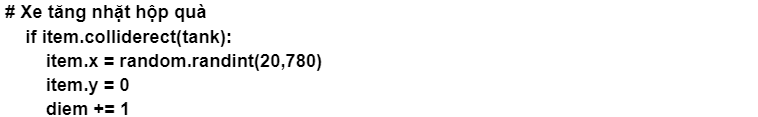
\includegraphics[width=5.5in,height=0.8in]{image13_2.png}

Trong trò chơi, khi xe tăng nhặt hộp quà, vị trí của hộp quà sẽ được
thiết lập ngẫu nhiên trên trục x và điểm số của người chơi tăng lên.
Điều này tạo ra cơ chế nhặt hộp quà để người chơi tăng điểm khi chơi trò
chơi.

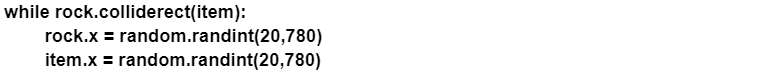
\includegraphics[width=5.5in,height=0.6in]{image13_3.png}

Ta dùng hàm random để hộp quà xuất hiện ngẫu nhiên theo trục Ox tức là
theo chiều ngang, hộp quà sẽ xuất hiện tại vị trí đầu của trục Oy và rơi
xuống, xử lý việc khi thiên thạch (rock) va chạm với hộp quà (item)
trong trò chơi.

Việc xử lý này giúp tránh tình huống thiên thạch và hộp quà va chạm với
nhau, khi đó chúng sẽ được đặt lại vị trí ngẫu nhiên trên màn hình. Điều
này giúp tránh tình trạng va chạm liên tục giữa hai đối tượng và tạo ra
một trải nghiệm chơi game mượt mà hơn.

\textbf{Lưu ý:} để tránh trường hợp hàm random hoạt động sai, ví dụ
chúng random các hộp quà ra khỏi kích thước của bản đồ, ta phải giới hạn
vị trí của chúng.

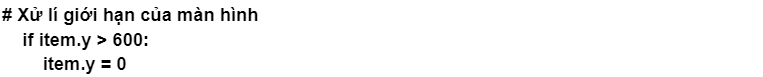
\includegraphics[width=5.5in,height=0.6in]{image13_4.png}

Xử lý giới hạn màn hình trong một ứng dụng hoặc trò chơi. Nó kiểm tra
xem một vật phẩm \textbf{(item)} có vượt quá giới hạn dưới của màn hình không.
Nếu tọa độ y của vật phẩm lớn hơn \textbf{600} (giả sử \textbf{600} là giới hạn dưới củamàn hình), nó sẽ đặt lại tọa độ y của vật phẩm thành \textbf{0}, làm cho vật phẩmxuất hiện trở lại ở phía trên màn hình. Điều này giúp giữ cho vật phẩmkhông bị "mất" khỏi màn hình khi nó di chuyển xuống quá nhanh.
\subsubsection{Xử lí khi xe tăng va trúng thiên thạch}
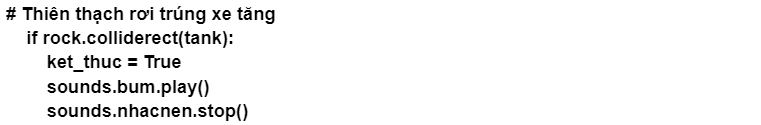
\includegraphics[width=5.5in,height=0.8in]{image13_5.png}

Khi một thiên thạch va chạm với xe tăng, trò chơi sẽ kết thúc. Âm thanh
"bum" sẽ phát ra và nhạc nền sẽ được dừng để tạo hiệu ứng cảm xúc và tập
trung vào âm thanh va chạm.

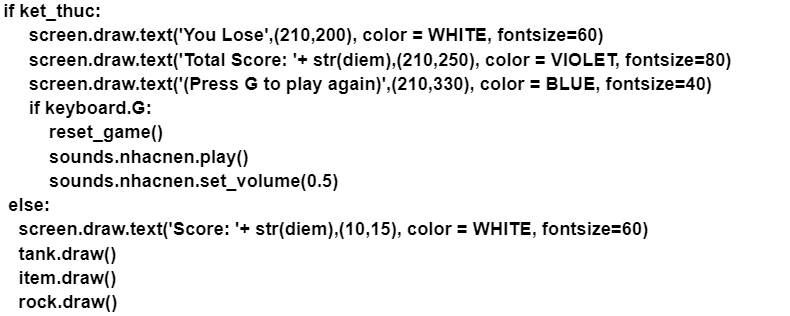
\includegraphics[width=6in,height=2in]{image13_6.png}

Nếu trò chơi kết thúc, thông báo \textbf{"You Lose"} sẽ được hiển thị
cùng với điểm số tổng cộng và hướng dẫn chơi lại. Nếu người chơi nhấn
\textbf{phím "G"}, trò chơi sẽ được thiết lập lại và nhạc nền sẽ được phát lại. Nếu trò chơi đang diễn ra, điểm số hiện tại sẽ được hiển thị và các đối tượng trò chơi sẽ xuất hiện trên màn hình.

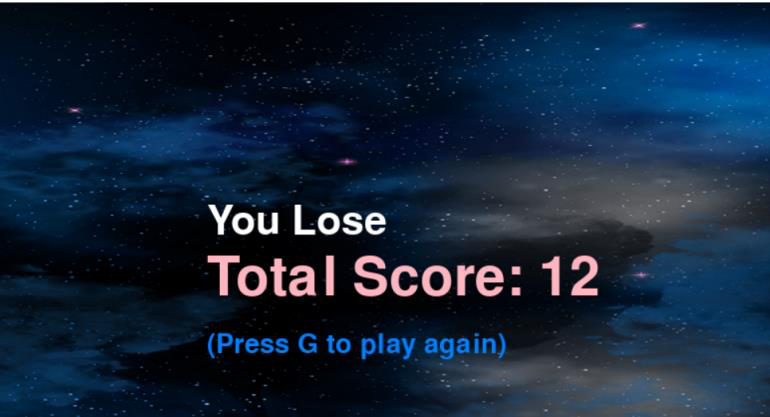
\includegraphics[width=3.49861in,height=1.89305in]{image14.png}

\subsubsection{Xử lí cửa sổ game}
Trước khi chạy game, set up vị trí cho cửa sổ lúc nó hiện lên sẽ nằm
phía trên và ở giữa

Thực hiện thiết lập biến môi trường \textbf{SDL\_VIDEO\_CENTERED} thành
1 và biến môi trường \textbf{SDL\_VIDEO\_WINDOW\_POS} thành một chuỗi
thể hiện vị trí cửa sổ mong muốn.

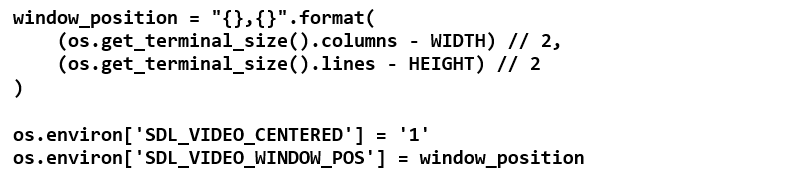
\includegraphics[width=5in,height=1in]{image14_1.png}

Sử dụng biến môi trường \textbf{SDL\_VIDEO\_CENTERED} và
\textbf{SDL\_VIDEO\_WINDOW\_POS} để căn giữa cửa sổ đồ họa trong thiết bị đầu cuối. Điều này đảm bảo cửa sổ được tạo sẽ hiển thị ở vị trí căn giữa trên thiết bị đầu cuối.

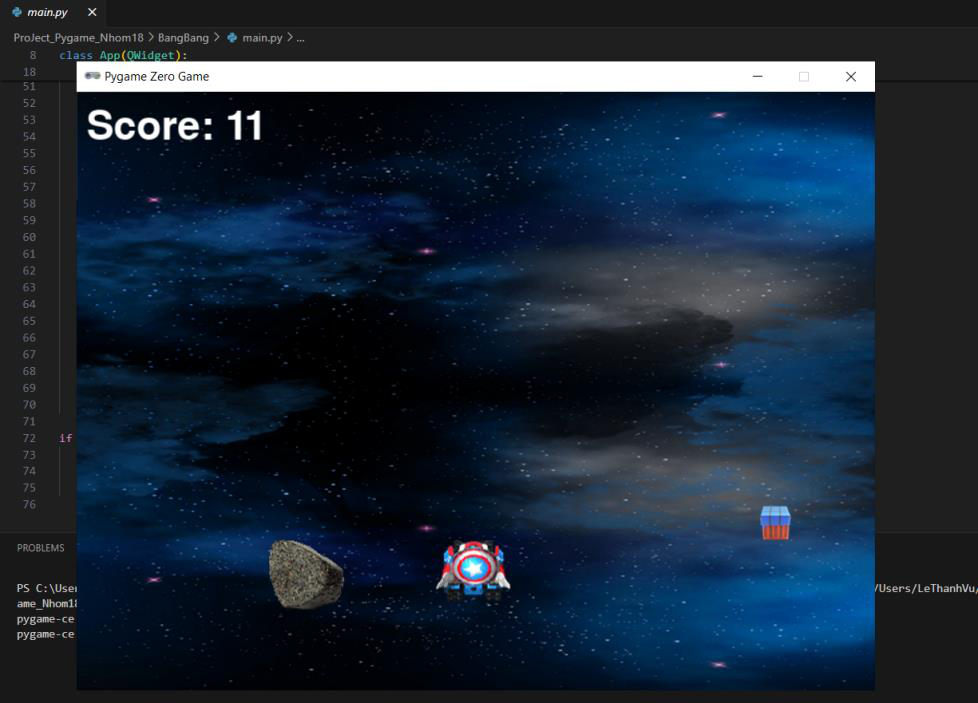
\includegraphics[width=4.44305in,height=3.19722in]{image15.png}
\subsubsection{Hiệu ứng âm thanh}
Nhạc nền: \textbf{sounds.nhacnen.play()}\\
Âm lượng nhạc nền: \textbf{sounds.nhacnen.set\_volume(0.5)} Va vào thiên
thạch: \textbf{sounds.bum.play()}\\
Ngừng nhạc nền: \textbf{sounds.nhacnen.stop()}
\newpage
\section{MODE TANK PVP}
Nhắc đến trò chơi điện tử (hay game), chắc chắn không ai xa lạ với thuật
ngữ này, đây là thứ gắn liền với tuổi thơ của biết bao thế hệ, gắn bó
với mọi người, chắc chắn ai cũng từng chơi qua một lần. Dạng sơ khai
nhất của game chính là các trò chơi như cờ caro được chơi trên giấy, cờ
vua, cờ tướng,... Hiện nay trò chơi đã được nâng lên một tầm cao mới, từ
khi công nghệ cũng như internet phát triển, các lập trình viên đã mô
hình hóa và đưa thành công nó lên các nền tảng thiết bị điện tử. Ngày
nay trò chơi điện tử đã không ngừng được cải thiện lối chơi, đồ họa, các
thể loại ngày càng hấp dẫn, thu hút đông đảo giới trẻ yêu thích. Khi nói
đến game thì nhiều người thường nghĩ rằng nó là một thứ vô bổ, lãng phí
thời gian, ảnh hưởng đến health và học tập. Và dĩ nhiên ở chiều ngược
lại, các nhà khoa học đã chứng minh rằng, nếu chơi game điều độ, có
chừng mực thì sẽ giúp nhóm em xả stress sau những giờ học tập và làm
việc căng thẳng, và đối với một số tựa game như Minecraft, Lego còn
khiến nhóm em rèn luyện khả năng tư duy sáng tạo cho trẻ.

Trong thế giới hỗn loạn và đầy cạnh tranh này, chào mừng bạn đến với đấu
trường PvP hoành tráng, nơi kỹ năng, chiến lược và lòng dũng cảm sẽ được
thử thách đến cùng cực. Hãy sẵn sàng đọ sức với những đối thủ ngang tài
ngang sức, chứng minh bản lĩnh và vươn lên dẫn đầu bảng xếp hạng. Với
nhiều chế độ chơi đa dạng, từ đấu đội 5v5 căng thẳng đến đấu đơn 1v1 gay cấn, tựa game tank PvP của nhóm mình mang đến trải nghiệm chơi game đỉnh cao cho mọi game thủ. Tùy chỉnh nhân vật của bạn, trang bị cho họ những vũ khí và áo giáp mạnh mẽ nhất, và bước vào đấu trường để chiến đấu vì vinh quang và phần thưởng. Cho dù bạn là một chiến binh dày dạn kinh nxuấtệm hay một tân binh háo hức, đấu trường PvP luôn chào đón bạn. Hãy rèn luyện kỹ năng của mình, lập nhóm với bạn bè và chứng minh rằng bạn có những gì cần thiết để trở thành nhà vô địch tối thượng.

Tham gia ngay vào tựa game \textbf{PvP} của nhóm mình và trải nxuấtệm
cảm giác hồi hộp khi chiến đấu với những người chơi khác trong thời gian
thực. Vinh quang đang chờ đón những người dũng cảm nhất. Hãy sẵn sàng
cho trận chiến và chứng minh sức mạnh của bạn!

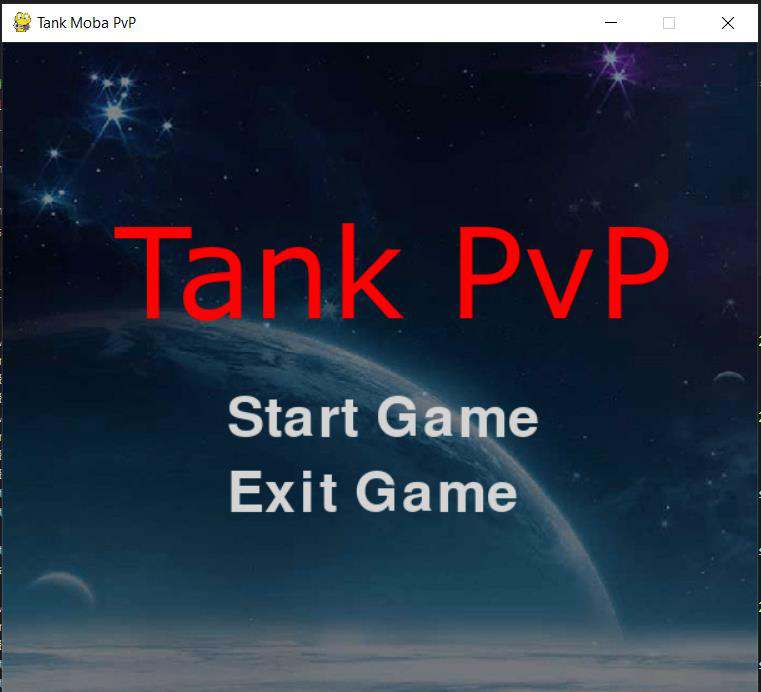
\includegraphics[width=4.50833in,height=4.1in]{image16.png}
\subsection{Hướng dẫn cách chơi}
Click \textbf{Start Game} để bắt đầu trò chơi.


\includegraphics[width=4.28056in,height=1.03194in]{image17.png}

Đến phần chọn tank và phần hướng dẫn dành cho người chơi 1 và người chơi 2.

Đối với người chơi 1 thì sẽ sử dụng các phím chức năng \textbf{W A S D}
để di chuyển lên, xuống, trái, phải. Phím bắn đạn sẽ là phím số 4.

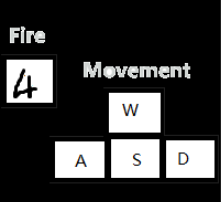
\includegraphics[width=1.77778in,height=1.625in]{image18.png}

Đối với người chơi 2 thì sẽ sử dụng các phím mũi tên (hãy bật
\textbf{scroll lock} nếu bạn không di chuyển được) để di chuyển lên,
xuống, trái, phải.

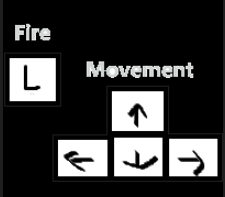
\includegraphics[width=2.34306in,height=2.05278in]{image19.png}

Tiến hành chọn tank:


\includegraphics[width=4.20694in,height=1.03194in]{image20.png}

Đối với người chơi 1 thì dùng phím \textbf{A và D} để di chuyển qua lại
chọn tank yêu thích.

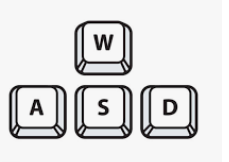
\includegraphics[width=2.38333in,height=1.6875in]{image21.png}

Đối với người chơi 2 thì dùng phím \textbf{mũi tên} → để di chuyển qua lại chọn tank yêu thích.

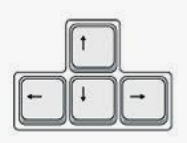
\includegraphics[width=1.94583in,height=1.48889in]{image22.png}

Tùy theo loại tank, mỗi loại đều có chỉ số khác nhau đảm bảo công bằng
khi chơi:\\
-Loại tank ver1 sẽ có ít máu, nhưng tốc độ nhanh, tốc độ nạp đạn chậm

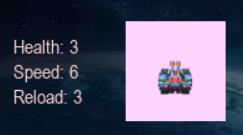
\includegraphics[width=2.52917in,height=1.40555in]{image23.png}

-Loại tank ver2 sẽ có nhiều máu hơn, nhưng tốc độ chậm, tốc độ nạp đạn
nhanh.

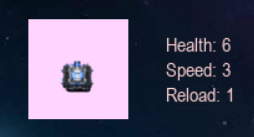
\includegraphics[width=2.64444in,height=1.42639in]{image24.png}

\subsection{Ý tưởng thực hiện}
Nhóm quyết định phân chia từng phần của trò chơi thành các hàm riêng
biệt do dự án có quy mô khá lớn. Phương pháp này giúp việc giải thích và
ghi chú trở nên dễ dàng hơn. Dưới đây là một mô tả tổng quan về
pseudocode của trò chơi của chúng tôi. Thông qua việc sử dụng pseudocode
và phân chia trò chơi thành các hàm riêng biệt, chúng tôi hy vọng rằng
việc hiểu và duy trì mã nguồn của trò chơi sẽ dễ dàng hơn, đồng thời
cũng giúp tối ưu hóa quá trình phát triển.

Quá trình chuẩn bị cho trò chơi bắt đầu bằng việc import thư viện
pygame, khởi động Pygame, thiết lập Pygame Mixer cho âm thanh, khởi tạo
màu sắc và biến font. Sau đó, tạo cửa sổ trò chơi, thiết kế hình nền,
nạp âm thanh, hình ảnh bản đồ và xe tăng, đặt điểm xuất hiện xe tăng,
tạo nhóm người chơi, nhân vật, thêm xe tăng, quản lý tường và viên đạn,
và cuối cùng đặt biến điều khiển cho hàm và vòng lặp trong trò chơi.

Nhóm sẽ ghi điểm vào file điểm khi có, thiết lập số khung hình trên giây
để chạy mượt mà, gọi hàm menu để hiển thị giao diện người chơi và xử lý
sự kiện chuột. Khi người dùng chọn "chơi trò chơi", hàm menu sẽ kết thúc
và dừng phát nhạc nền. Khi chọn "thoát trò chơi", hàm menu sẽ kết thúc,
đặt giá trị false cho biến điều khiển và dừng phát nhạc.

Nhóm tải và phát nhạc nền khi call màn hình lựa chọn xe tăng, hiển thị
tên các mục lựa chọn và hình ảnh, yêu cầu người chơi sử dụng phím điều
khiển để chuyển đổi xe tăng. Khi người chơi nhấn Enter, xác nhận xe tăng
được chọn và cập nhật thông số. Sau đó, chọn bản đồ và kết thúc hàm lựa
chọn. Nếu người chơi thoát, hàm sẽ kết thúc và dừng phát nhạc.

Nhóm hẹn giờ cho việc bắn đạn khi màn hình chiến đấu được kích hoạt, sau
đó nạp và phát nhạc nền. Trong vòng lặp, họ di chuyển người chơi, xử lý
việc bắn đạn và đóng cửa sổ trò chơi. Duyệt qua đạn để xử lý va chạm và
hiển thị trạng thái trên màn hình. Khi sức khỏe của người chơi giảm về
0, kết thúc trò chơi và dừng nhạc nền.

Nhóm sẽ tải và phát nhạc nền khi hàm kết thúc trò chơi được gọi, sau đó
cập nhật điểm số từ tệp và xác định người chiến thắng. Người chiến thắng
sẽ được cộng thêm một điểm và điểm số mới sẽ được ghi lại. Tiêu đề kết
quả sẽ được hiển thị trên màn hình và trong vòng lặp, điểm số sẽ được
hiển thị và xử lý sự kiện như dừng phát nhạc, thiết lập lại điểm số hoặc
kết thúc trò chơi sẽ được thực hiện.

Tạo ra một vùng trống bị giới hạn bởi rìa bản đồ, sau đó thiết lập hai
đối thủ (ta và địch), mỗi đối tượng sẽ đặt ở 2 góc bản đồ. Đưa xe tăng
của hai người chơi lên bản đồ, player 1 đặt ở góc trái bên trên map,
player 2 đặt ở góc dưới bên phải map.

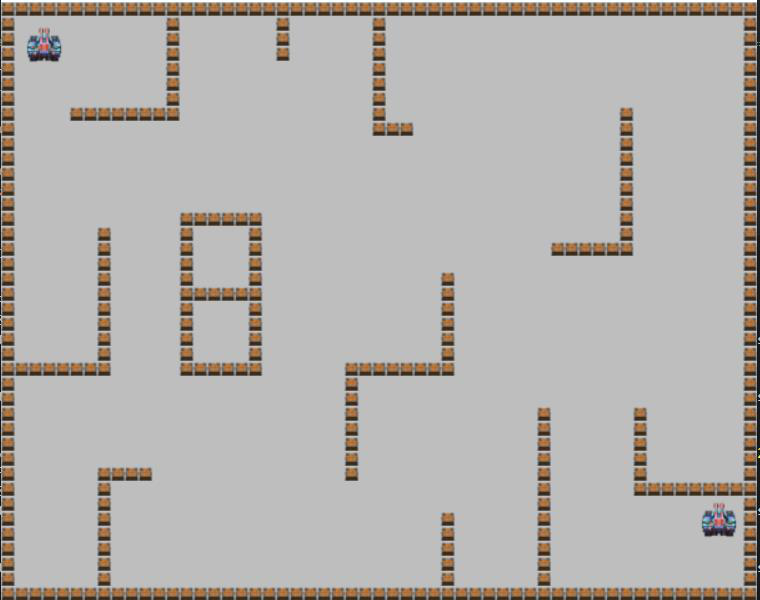
\includegraphics[width=3.58889in,height=2.83333in]{image25.png}

Sau đó 2 chiếc xe tăng sẽ đối đầu lẫn nhau bằng cách bắn đạn nhằm hạ gục
đối phương, đồng thời cố gắng di chuyển để né đạn từ địch.

Để tạo ra một trải nxuấtệm chơi đầy sinh động và hấp dẫn hơn, nhóm em sẽ
thiết kế các vách tường gỗ đặc biệt, những bức tường chắn đạn sẽ ngăn
cản việc bắn trực tiếp vào nhau. Điều này sẽ tạo ra các tình huống chiến
đấu trong game trở nên chân thực hơn, khi người chơi phải tìm cách vượt
qua các vách tường này để tiến xa hơn trong trận đấu

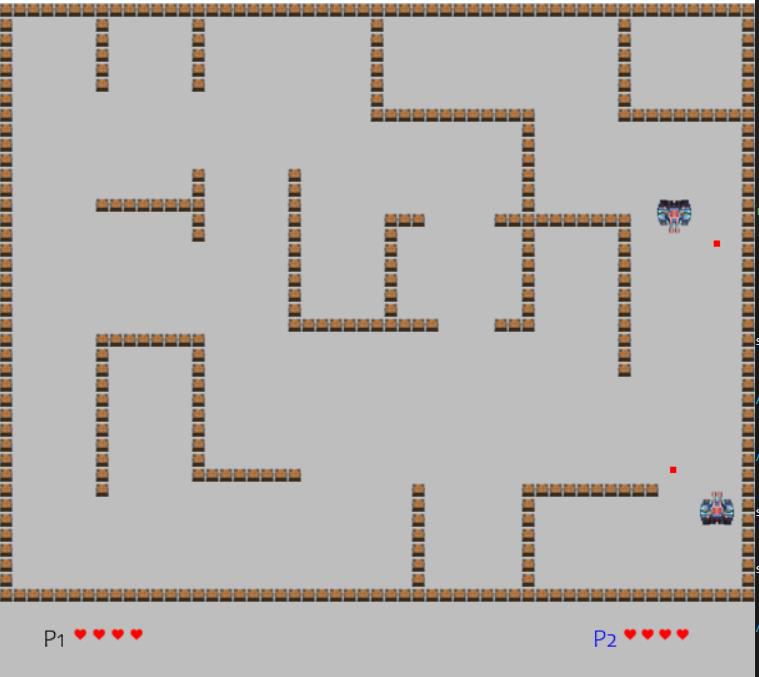
\includegraphics[width=3.58194in,height=3.19583in]{image26.png}
\newpage
\subsection{Mô hình hóa chương trình}
\subsubsection{Mô tả chi tiết các thành phần cần xử lí}
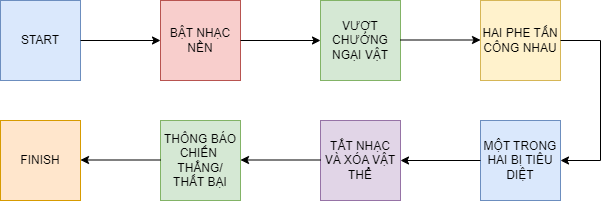
\includegraphics[width=5.53194in,height=1.82222in]{image27.png}
\subsubsection{Cơ chế quá trình hoạt động}
-\textbf{Căn chỉnh cửa sổ, kích thước, định dạng xe tăng của người
chơi:}

+ Căn chỉnh cửa sổ hiển thị để đảm bảo rằng mọi thành phần trên giao
diện game được hiển thị một cách rõ ràng và hợp lý.

+ Xử lý việc kích thước của cửa sổ và các thành phần bên trong để đảm
bảo sự cân đối và thuận tiện cho người chơi.

+ Định dạng xe tăng của người chơi, bao gồm việc thiết kế và hiển thị xe
tăng một cách chân thực và đáng tin cậy trong game.

+ Cơ chế điều khiển sẽ bao gồm việc sử dụng bàn phím để thực hiện các
hành động trong trò chơi.

+ Hướng di chuyển của tank sẽ phụ thuộc vào cách người chơi sử dụng các
phím điều khiển để di chuyển lên, xuống, trái, phải hay các phím
\textbf{W A S D.}

+ Vị trí ban đầu của các tank trên bản đồ sẽ được xác định trước khi trò
chơi bắt đầu, là ở các vị trí ngẫu nhiên hoặc được đặt sẵn để tạo ra sự
cân bằng và chiến lược cho người chơi.

-\textbf{Thiết lập cơ chế đạn của người chơi:}

+ Cơ chế phím bắn của đạn sẽ xử lý việc người chơi sử dụng phím cụ thể
để bắn đạn từ xe tăng của mình.

+ Hướng bay của đạn sẽ phụ thuộc vào hướng mà người chơi di chuyển xe
tăng và hướng bắn, đảm bảo tính chính xác và logic của việc bắn đạn. +
Vị trí theo xe tăng khi bắn đạn sẽ xác định vị trí xuất phát của đạn từ
xe tăng, đồng thời cũng ảnh hưởng đến quỹ đạo di chuyển của đạn.

+ Xử lý loại bỏ đạn khi chúng trúng vào tường hay trúng vào đối thủ để
đảm bảo tính logic và hiệu quả của trò chơi.

+ Viên đạn sẽ di chuyển theo hướng được xác định bởi thuộc tính
direction của nó.

+ Trong mỗi lần cập nhật, viên đạn sẽ di chuyển một khoảng cố định trên
màn hình game dựa trên hướng của nó: sang trái, sang phải, lên trên hoặc
xuống dưới.

+ Đối với hướng di chuyển sang trái hoặc lên trên, tọa độ của viên đạn
sẽ giảm để thực hiện di chuyển.

+ Đối với hướng di chuyển sang phải hoặc xuống dưới, tọa độ của viên đạn
sẽ tăng để thực hiện di chuyển.

+ Khoảng cách di chuyển mỗi lần là 6 pixel theo phương ngang hoặc dọc
tương ứng với hướng bắn của đạn.

-\textbf{Định dạng xe tăng của hai người chơi;}

+ Để cài đặt cơ chế tự điều khiển, nhóm em cần xử lý việc lập trình để
xác

định hành vi tự động của các vật thể trong trò chơi, bao gồm việc di
chuyển, tấn công và phòng thủ.

+ Cơ chế xoay hướng sẽ giúp tank trong trò chơi tự động nhận biết và
phản

ứng với các tình huống xung quanh, bao gồm việc xoay hướng để tấn công
hoặc tránh né đạn của đối thủ.

+ Vị trí ban đầu trên map và khoảng cách giữa hai người chơi với nhau sẽ

ảnh hưởng đến chiến thuật và cách tiếp cận trong trò chơi, cần được xác
định một cách cân nhắc để tạo ra trải nxuấtệm chơi game hấp dẫn và thú
vị.

-\textbf{Thiết lập cơ chế bắn đạn của hai người chơi:}

+ Xác định các phím điều khiển cho việc bắn đạn của từng người chơi, ví
dụ: người chơi 1 sử dụng phím 4 và người chơi 2 sử dụng phím L.

+ Khi người chơi thực hiện hành động bắn, hàm sẽ tạo ra viên đạn. Kích
thước của viên đạn được thiết lập là 5x5 pixel.

+ Màu sắc của đạn chủ yếu là đỏ với giá trị RGB là (255,0,0).

+ Vị trí ban đầu của viên đạn được thiết lập tùy theo hướng mà tank của
người chơi đang quay mặt: lên trên, xuống dưới, sang trái, hay sang
phải.

+ Viên đạn sẽ được đặt tại một vị trí sao cho vừa khít với giữa nòng
súng tank khi nó được bắn ra.

+ Sau khi thiết lập, viên đạn sẽ được thêm vào nhóm các đối tượng đạn đã
được tạo sẵn trong trò chơi để quản lý.

+ Thiết lập hướng bắn và vận tốc đạn dựa trên hướng mà người chơi đặt xe
tăng của mình và hướng bắn từ các phím điều khiển tương ứng.

+ Xử lý va chạm giữa đạn của hai người chơi để xác định việc trúng đích
và xuất điểm.

+ Đảm bảo tính cân bằng giữa cơ chế bắn đạn của hai người chơi để tạo ra
trải nxuấtệm chơi game công bằng và hấp dẫn.

-\textbf{Xuất thông báo ra màn hình khi có một người chơi chiến thắng
hoặc thua:}

\textbf{+} Đọc số điểm của hai người chơi từ file BangTinhDiem.txt, lưu
trữ dưới dạng dictionary với key là tên người chơi và value là số điểm
đã chuyển thành số nguyên.

+ So sánh lượng máu còn lại của hai người chơi để xác định người thắng
cuộc (người còn nhiều máu hơn).

+ Hiển thị thông báo "PLAYER 1 WINS" với màu sắc cụ thể nếu người chơi 1
thắng, và tương tự, thông báo "PLAYER 2 WINS" nếu người chơi 2 thắng.
Thông báo này được hiển thị với màu vàng.

+ Cập nhật điểm số trong dictionary cho người chơi chiến thắng bằng cách
tăng số điểm của họ lên 1.

+ Xuất điểm số mới được cập nhật vào file BangTinhDiem.txt.

+ Hiển thị tiêu đề "END OF THE MATCH" với màu đỏ để cho biết trận đấu đã
kết thúc.

+ Hiển thị tiêu đề "Scores" với màu tím hồng, thông báo điểm số hiện tại
của cả hai người chơi.

+ Xuất thông báo hướng dẫn "Press R to reset scores!" với màu vàng,
hướng dẫn người chơi nếu muốn đặt lại điểm số.

+ Xuất thông báo hướng dẫn "Press ENTER to return to game menu." với màu
vàng, hướng dẫn người chơi quay trở lại menu chính của trò chơi.

-\textbf{Thêm vào các hiệu ứng như âm thanh, giao diện (nếu có):}

+ Bật nhạc nền khi vào game và tắt khi kết thúc game:\\
Khi vào game sử dụng hàm, thư viện âm thanh để phát nhạc nền.

Khi kết thúc game, dừng phát nhạc nền.

+ Phát ra âm thanh khi ta hoặc địch bắn:\\
Khi người chơi bắn, nhóm em sử dụng hàm, thư viện âm thanh để phát ra âm
thanh tương ứng.

+ Phát ra âm thanh khi người chơi bị trúng đạn:

Khi kẻ địch hoặc người chơi bị trúng đạn, nhóm em cũng sử dụng hàm thư
viện âm thanh để phát ra âm thanh báo hiệu.

Bằng cách này, việc sử dụng âm thanh trong trò chơi không chỉ tạo ra
trải nxuấtệm âm nhạc hấp dẫn mà còn giúp người chơi dễ dàng nhận biết
các tình huống quan trọng trong trò chơi.
\newpage
\subsection{Quy trình thực hiện}
\subsubsection{Thư viện cần dùng}
\textbf{import Math import pygame}\\
\textbf{from pygame.locals import *}\\
\textbf{import random}\\
\textbf{import time}\\
\textbf{pygame.init()}

- \textbf{Math}: Thư viện toán học chuẩn của Python, cung cấp các hàm
toán học như lũy thừa, căn bậc hai, các hàm lượng giác, v.v.

- \textbf{pygame}: Thư viện chuyên cho việc phát triển trò chơi, hỗ trợ
tạo cửa sổ, xử lý đồ họa, âm thanh, và xử lý sự kiện.

- \textbf{from pygame.locals import} : Nhập tất cả các hằng số có sẵn từ
module \textbf{pygame.locals}, thường được sử dụng để dễ dàng tham chiếu
tới các nút bấm, hằng số hệ thống mà không cần phải gọi module
\textbf{pygame.locals.}

- \textbf{random}: Thư viện hỗ trợ tạo ra các số ngẫu nhiên, sử dụng cho
việc lựa chọn ngẫu nhiên, xáo trộn dữ liệu, v.v.

- \textbf{time}: Thư viện cung cấp các hàm để làm việc với thời gian,
bao gồm đo hạn, đợi (sleep), và xuất lại thời gian hệ thống, v.v.

Với dòng lệnh \textbf{pygame.init()}, thư viện pygame được khởi tạo, đây
là bước cần thiết để bắt đầu làm việc với pygame.
\subsubsection{Căn chỉnh cửa sổ}
\textbf{size = (605, 540) \#kích thước cửa sổ game}\\
\textbf{screen = pygame.display.set\_mode(size)}\\
\textbf{screenPIC =}\\
\textbf{pygame.image.load(\textquotesingle ProJect\_Pygame\_Nhom18/BangBang/Tank2P/picture/anhn
en.png\textquotesingle)}\\
\textbf{pygame.display.set\_caption("Tank PvP Group\_18'')}\\
\textbf{background = pygame.Surface(size)}\\
\textbf{background = background.convert()}\\
\textbf{background.fill(colours{[}\textquotesingle grey\textquotesingle{]})}

- Thiết lập kích thước cửa sổ game là \textbf{605x540 pixel.}

- Tạo màn hình hiển thị với kích thước đã thiết lập.

- Tải hình ảnh nền từ đường dẫn\\
\textbf{\textquotesingle ProJectPygameNhom18/BangBang/Tank2P/picture/anhnen.png\textquotesingle{}}
và lưu vào biến \textbf{screenPIC.}

- Đặt tiêu đề cửa sổ game là \textbf{"Tank PvP Group\_18".}

- Tạo một đối tượng \textbf{Surface} mới với kích thước cửa sổ game.

- Chuyển đổi đối tượng \textbf{Surface} vừa tạo để tối ưu hiệu suất hiển
thị.

- Điền màu nền cho đối tượng \textbf{Surface} này bằng giá trị màu
\textquotesingle grey\textquotesingle{} từ dictionary màu colours.

Ở đây ta chọn kích thước của cửa sổ chương trình, trong đó chiều dài và

chiều rộng lần lượt là \textbf{605 x540}, đây là kích thước tiêu chuẩn
cho game 2D, ngoài ra còn phù hợp với kích thước của hình nền.

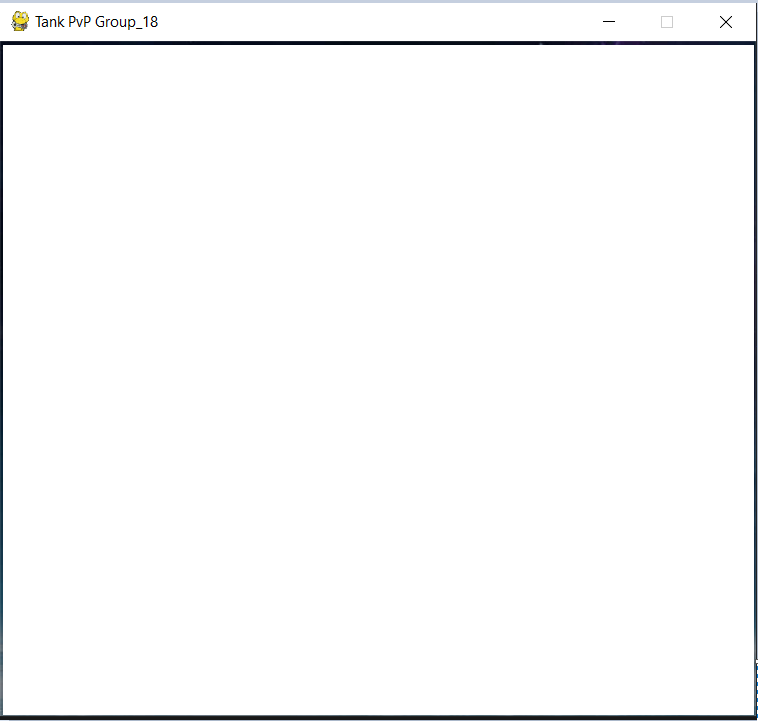
\includegraphics[width=4.85278in,height=4.61667in]{image28.png}

\subsubsection{Thiết kế giao diện menu game}
Xử lý sự kiện cho lựa chọn của người chơi trong menu game thông qua click chuột, tập trung vào tương tác chuột và chức năng thoát. Nó xác định các hàm để tăng cường menu game bằng cách thiết lập nhạc nền, hiển thị tiêu đề game với các lựa chọn \textbf{"Start Game"} và \textbf{"Exit Game"} được làm nổi bật khi di chuột qua, quản lý sự kiện chuột để bắt đầu hoặc thoát game dựa trên lựa chọn của người chơi. Nó cũng bao gồm việc tải và phát nhạc nền, xuất tiêu đề game \textbf{"Tank PvP"} màu đỏ, tạo và đặt các nút \textbf{"Start} \textbf{Game"} và \textbf{"Exit Game"} trên màn hình. Sử dụng vòng lặp
while để theo dõi vị trí chuột, thay đổi hiệu ứng văn bản cho lựa chọn
dựa trên vị trí chuột của người chơi, xuất nền và văn bản trò chơi trên
màn hình, và cập nhật hiển thị.

Việc thiết lập cơ bản của hàm gameMenu tạo nền tảng cho một màn hình
menu thân thiện với người dùng và hấp dẫn về mặt hình ảnh. Bằng cách kết
hợp các yếu tố động, cải thiện âm thanh và hình ảnh, và tính năng tương
tác, người chơi được cung cấp một chuyển đổi mượt mà vào trải nxuấtệm
chơi game. Thiết kế chu đáo này không chỉ tối ưu hóa điều hướng mà còn
tạo ra không khí cho một phiên chơi game sâu sắc.
\subsubsubsection{Khởi tạo và hiển thị menu game}
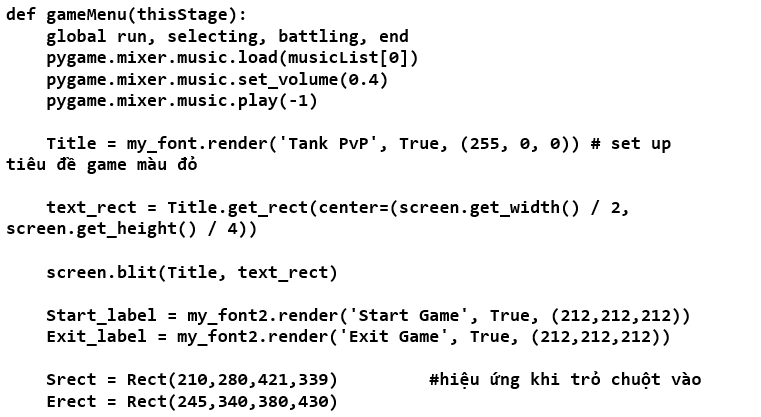
\includegraphics[width=6in,height=3in]{image28_1.png}

Hàm \textbf{gameMenu} trong ứng dụng \textbf{Pygame} đóng vai trò quan trọng trong việc thiết lập màn hình \textbf{menu} chính cho trò chơi. Ở trung tâm của hàm \textbf{gameMenu} là tham số \textbf{thisStage}, cho phép xác định các giai đoạn hoặc trạng thái cụ thể trong giao diện \textbf{menu}. Tham số này phục vụ như một yếu tố linh hoạt thích ứng với tương tác của người dùng, hướng dẫn họ qua menu một cách mượt mà.

Việc khai báo các biến toàn cục như \textbf{run}, \textbf{selecting}, \textbf{battling} và \textbf{end} cung cấp cho hàm sự linh hoạt để sửa đổi các giá trị này trong quá trình thực thi. Những biến này hoạt động như các cờ kiểm soát, ảnh hưởng đến hành vi của \textbf{menu} dựa trên đầu vào của người dùng và sự kiện hệ thống.

Kết hợp âm nhạc vào trải nghiệm chơi game tăng cường không khí tổng
thể. Bằng cách tải bản nhạc khởi đầu từ musicList và đặt âm lượng của nó
là \textbf{0.4}, hàm \textbf{gameMenu} tạo điều kiện cho một bản nhạc nền hấp dẫn. Bắt đầu phát nhạc trong một vòng lặp đảm bảo một bản nhạc liên tục và cuốn hút suốt quá trình tương tác với \textbf{menu}. Các yếu tố hình ảnh của menu đóng vai trò quan trọng trong việc thu hút sự chú ý của người chơi. Tạo một bề mặt cho tiêu đề "\textbf{Tank PvP}" với màu đỏ nổi bật không chỉ thu hút mắt mà còn xác định danh tính của trò chơi. Đặt tiêu đề ở giữa màn hình tăng cường sự nổi bật của nó, biến nó thành một điểm trọng tâm cho người
chơi.

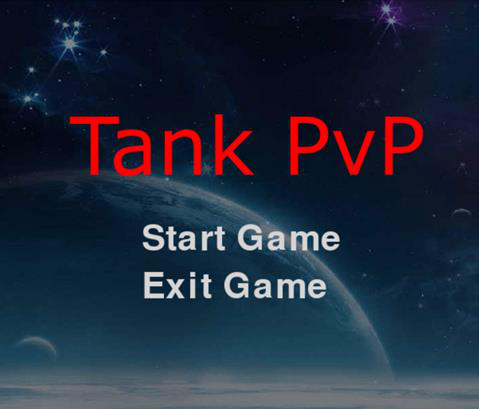
\includegraphics[width=4.98889in,height=4.26111in]{image29.png}

Việc bổ sung các yếu tố tương tác như nhãn \textbf{Start Game} và \textbf{Exit Game} thêm
chức năng vào menu. Những văn bản này, hiển thị trong \textbf{gam màu
xám} tinh tế, khuyến khích người chơi bắt đầu trò chơi hoặc thoát ứng
dụng. Ngoài ra, xác định các vùng hình chữ nhật (\textbf{Srect} và \textbf{Erect}) cho phép phát hiện hover và click, hỗ trợ tương tác và phản hồi từ người dùng.

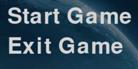
\includegraphics[width=1.4375in,height=0.71944in]{image30.png}
\newpage
\subsubsubsection{Xử lý sự kiện thoát khỏi game và chọn tùy chọn trong menu}
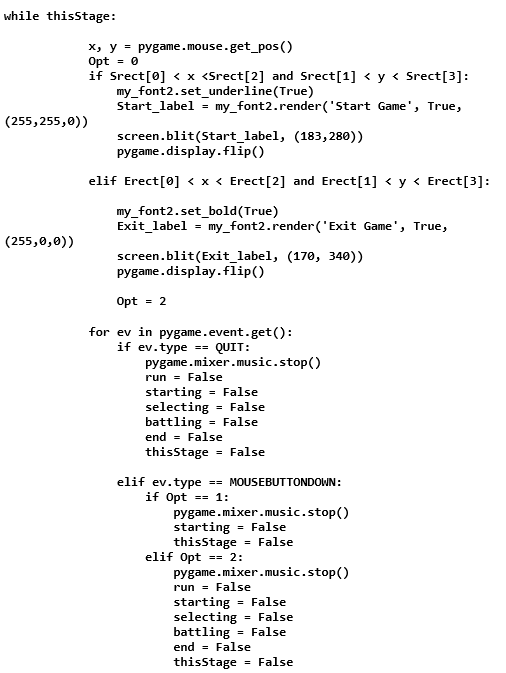
\includegraphics[width=5in,height=7in]{image30_1.png}
\newpage
Thiết lập của vòng lặp cho menu trò chơi. Quản lý việc hiển thị và tương
tác của người dùng với menu chính, xử lý việc bắt đầu hay thoát trò chơi
dựa trên đầu vào từ chuột. Trong vòng lặp while này, các sự kiện chuột
và tương tác người dùng được xử lý:

- Hàm \textbf{pygame.mouse.get\_pos()} lấy vị trí hiện tại của con trỏ chuột.

- \textbf{Opt} được khởi tạo với giá trị \textbf{0}, có thể được sử dụng để theo dõi lựa chọn của người chơi trong menu.

- if \textbf{Srect{[}0{]} \textless{} x \textless{} Srect{[}2{]} and
Srect{[}1{]} \textless{} y \textless{} Srect{[}3{]}}: kiểm tra nếu con
trỏ chuột đang ở bên trên nút "\textbf{Start Game}". Nếu đúng, thì chữ "\textbf{Start Game}" được gắn dấu gạch dưới và màu của nó thay đổi thành màu vàng, được thể hiện bằng nhãn \textbf{Start\_label}.


\includegraphics[width=3.75833in,height=0.90555in]{image17.png}

- elif \textbf{Erect{[}0{]} \textless{} x \textless{} Erect{[}2{]} and
Erect{[}1{]} \textless{} y \textless{} Erect{[}3{]}}: thực hiện việc kiểm tra tương tự cho nút "\textbf{Exit Game}". Nếu đúng, thì chữ "\textbf{Exit Game}" được in đậm và màu đỏ, được thể hiện bằng nhãn \textbf{Exit\_label}. Biến Opt được thiết lập là 2.


\includegraphics[width=3.75972in,height=0.875in]{image31.png}

- Các thiết lập nền \textbf{(screen.blit(screenPIC, (0,0)))} và tiêu đề \textbf{(screen.blit(Title, (90,120)))} cùng với các nhãn "Start Game" và "\textbf{Exit Game}" được xuất lên màn hình, và màn hình được cập nhật liên tục bằng hàm \textbf{pygame.display.flip()}.

- Sau đó, các sự kiện từ \textbf{pygame.event.get()}. Nếu sự kiện là \textbf{QUIT}, nhạc nền sẽ dừng chơi và tất cả các \textbf{flag} như \textbf{run}, \textbf{starting}, \textbf{selecting}, \textbf{battling}, \textbf{end} và \textbf{thisStage} đều được thiết lập về \textbf{False}, vừa để dừng vòng lặp và vừa để thoát khỏi \textbf{menu}.

- Khi sự kiện \textbf{MOUSEBUTTONDOWN} (nhấp chuột) xảy ra, tuỳ thuộc vào biến
Opt mà hành động tiếp theo sẽ được quyết định:

+ Nếu \textbf{Opt} bằng 1 (có thể bạn không hiển thị đoạn code liên quan đến việc thiết lập Opt thành 1), có thể sẽ bắt đầu trò chơi.

+ Nếu \textbf{Opt} bằng 2, nhạc nền dừng chơi và tất cả các biến, tương tự như
trong sự kiện \textbf{QUIT}, được thiết lập về False để thoát kịp thời.
\subsubsection{Thiết lập màn hình Select Tank}
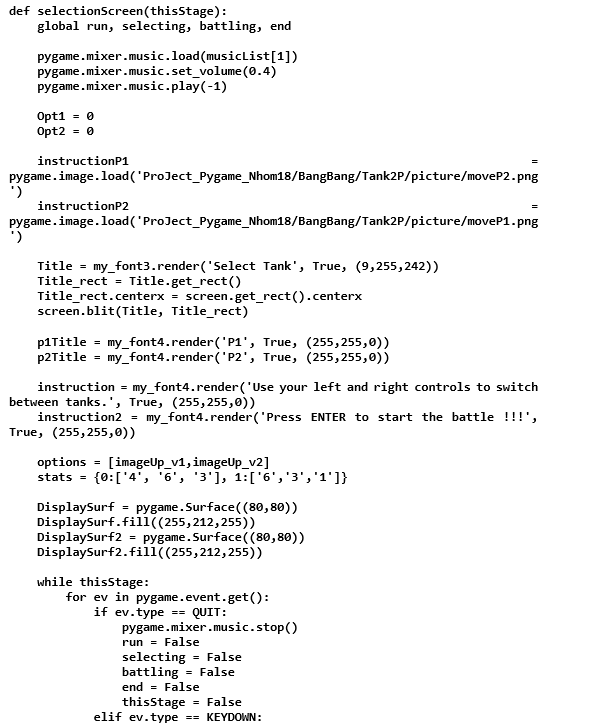
\includegraphics[width=5in,height=7in]{image30_2.png}

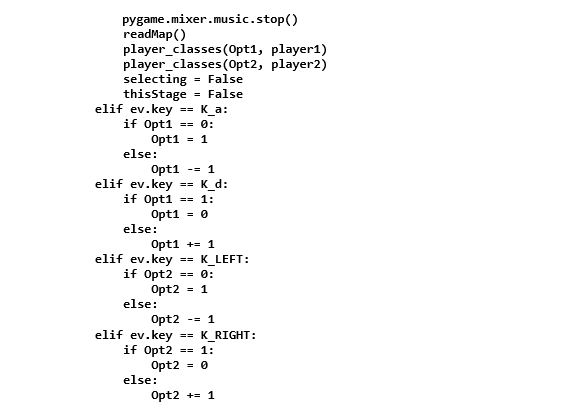
\includegraphics[width=6in,height=4.5in]{image30_3.png}

Quản lý quá trình chọn xe tăng và cài đặt các thông số trước khi bắt đầu
trò chơi. Lựa chọn và thao tác được thực hiện thông qua các phím điều
hướng và phím \textbf{ENTER}. Hàm này xử lý màn hình lựa chọn xe tăng
trước khi bắt đầu trận chiến.

\includegraphics[width=3.35833in,height=1.75in]{image32.png}

Ta thiết lập biến toàn cục gồm \textbf{run}, \textbf{selecting},
\textbf{battling}, và \textbf{end}. Hàm tải và phát nhạc nền từ
\textbf{musicList{[}1{]}} với âm lượng đã được đặt là 0.4 và lặp lại vô
hạn.

\textbf{Opt1} và \textbf{Opt2} được khởi tạo để lưu trữ lựa chọn xe tăng
của người chơi 1 và người chơi 2. Các hướng dẫn và tiêu đề cho người
chơi được tải và tạo từ các file ảnh và đối tượng font có sẵn.

Các biến như \textbf{Title}, \textbf{p1Title}, \textbf{p2Title},
\textbf{instruction}, và \textbf{instruction2} được tạo để hiển thị tiêu
đề màn hình lựa chọn, hướng dẫn người chơi v.v..., \textbf{options} là
mảng chứa hình ảnh đầu tiên (hình ảnh ở phía trên) của mỗi loại xe tăng
để người chơi lựa chọn. \textbf{Stats} là một từ điển chứa thông tin về
từng xe tăng, bao gồm "health," "tốc độ đạn," và "tốc độ di chuyển."
\textbf{DisplaySurf} và \textbf{DisplaySurf2} là các đối tượng
\textbf{Surface} được tạo ra để hiển thị thông tin về xe tăng được chọn;
chúng được tô màu để phân biệt.

\includegraphics[width=0.59306in,height=0.61389in]{image33.png}

Hàm chứa vòng lặp \textbf{whilethisStage} để tiếp tục hiển thị màn hình
lựa chọn cho đến khi người chơi hoàn tất việc lựa chọn hoặc thoát khỏi
game. Trong vòng lặp, hàm xử lý sự kiện từ \textbf{pygame.event.get()}:

- Nếu sự kiện là \textbf{QUIT}, nhạc nền sẽ dừng, tất cả các biến trạng
thái sẽ được đặt lại và \textbf{thisStage} sẽ trở thành \textbf{False}
để thoát khỏi màn hình lựa chọn.

- Nếu sự kiện là \textbf{KEYDOWN}, tuỳ thuộc vào phím được nhấn mà các
lựa chọn \textbf{Opt1} và \textbf{Opt2} (chỉ số lựa chọn xe tăng) sẽ
thay đổi:\\
- \textbf{K\_RETURN}: nhạc nền dừng, tải bản đồ game (\textbf{readMap()}
không được hiển thị trong đoạn vừa rồi nhưng giả định có liên quan đến
cài đặt trận chiến), áp dụng lựa chọn xe tăng vào đối tượng player1 và
player2 rồi thoát màn hình lựa chọn. - \textbf{K\_a} và \textbf{K\_d}:
thay đổi lựa chọn của người chơi 1 (P1).

- \textbf{K\_LEFT} và \textbf{K\_RIGHT}: thay đổi lựa chọn của người
chơi 2 (P2).

\includegraphics[width=6.3in,height=1.65in]{image34.png}
\newpage
\textbf{Tạo hiển thị thông tin tank và hướng dẫn:}

\includegraphics[width=6.5in, height=6in]{image34_1.png}

Người dùng thấy được tất cả những lựa chọn và thông tin liên quan trước
khi bắt đầu trận chiến, tạo nên giao diện người dùng cuối của màn hình
lựa chọn xe tăng trong game.

\includegraphics[width=3.66528in,height=2.56528in]{image35.png}
\newpage
\subsubsection{Định dạng xe tăng}
\textbf{players = pygame.sprite.Group()}\\
\textbf{player1 = pygame.sprite.Sprite()}\\
\textbf{player1.rect = pygame.Rect((20, 20),(24,24)) player1.direction =
\textquotesingle up\textquotesingle{}}\\
\textbf{player1.keys = (K\_a, K\_d, K\_w, K\_s,K\_4)}

\textbf{player2 = pygame.sprite.Sprite()}\\
\textbf{player2.rect = pygame.Rect((560, 390), (24,24))
player2.direction = \textquotesingle up\textquotesingle{}}\\
\textbf{player2.keys = (K\_LEFT, K\_RIGHT, K\_UP, K\_DOWN,K\_l)}

\textbf{players.add(player1)}\\
\textbf{players.add(player2)}

\textbf{bulletgroup = pygame.sprite.Group()}\\
\textbf{walls = pygame.sprite.Group()}

- Khai báo hai danh sách \textbf{ver1} và \textbf{ver2} chứa các hình
ảnh khác nhau cho hai phiên bản người chơi, với các hướng di chuyển khác
nhau được biểu diễn qua các hình ảnh lên, xuống, phải và trái.

\includegraphics[width=0.65417in,height=0.55972in]{image36.png}\includegraphics[width=0.43889in,height=0.5625in]{image37.png}\includegraphics[width=0.55833in,height=0.58333in]{image38.png}\includegraphics[width=0.54722in,height=0.60694in]{image39.png}

- Khởi tạo một danh sách \textbf{spawnpoints} chứa các vị trí xuất hiện
trên màn hình cho các viên đạn, mỗi vị trí được biểu diễn bởi một cặp
tuple chỉ định tọa độ x và y.

Sau đó code tiếp tục với việc tạo ra nhóm đối tượng:

- Tạo nhóm players sử dụng \textbf{pygame.sprite.Group()} để quản lý các
đối tượng người chơi.

- Tạo ra hai đối tượng player1 và player2 bằng cách sử dụng

\textbf{pygame.sprite.Sprite()}. Mỗi đối tượng người chơi được cấp một
hình chữ nhật (\textbf{rect}) để xác định vị trí và kích thước, một
thuộc tính \textbf{direction} để biết hướng di chuyển, và một set các
\textbf{keys} để xác định các phím điều khiển di chuyển và bắn đạn.

- Thêm hai đối tượng \textbf{player1} và \textbf{player2} vào nhóm
\textbf{players} bằng phương thức \textbf{add.}

\includegraphics[width=3.22639in,height=1.35694in]{image40.png}

Tiếp theo, code khởi tạo hai nhóm đối tượng khác:

- Nhóm \textbf{bulletgroup} sử dụng \textbf{pygame.sprite.Group()}, dùng
để quản lý các viên đạn trong trò chơi.

- Nhóm \textbf{walls} cũng dùng \textbf{pygame.sprite.Group()}, dùng để
quản lý các bức tường trong game.

Các nhóm này được sử dụng để quản lý và cập nhật trạng thái các đối
tượng tương ứng trong trò chơi, giúp dễ dàng thao tác xuất, kiểm tra va chạm
và xử lý sự kiện hơn.
\subsubsubsection{Định dạng và đưa hình ảnh 2 tank lên cửa sổ}
\textbf{imageUp\_v1 =}

\textbf{pygame.image.load(\textquotesingle ProJect\_Pygame\_Nhom18/BangBang/Tank2P/picture/tank1}

\textbf{up.png\textquotesingle)}

\textbf{imageDown\_v1 =}

\textbf{pygame.image.load(\textquotesingle ProJect\_Pygame\_Nhom18/BangBang/Tank2P/picture/tank1}

\textbf{down.png\textquotesingle)}

\textbf{imageRight\_v1 =}\\
\textbf{pygame.image.load(\textquotesingle ProJect\_Pygame\_Nhom18/BangBang/Tank2P/picture/tank1
right.png\textquotesingle)}\\
\textbf{imageLeft\_v1 =}\\
\textbf{pygame.image.load(\textquotesingle ProJect\_Pygame\_Nhom18/BangBang/Tank2P/picture/tank1
left.png\textquotesingle)}

\textbf{imageUp\_v2 =}\\
\textbf{pygame.image.load(\textquotesingle ProJect\_Pygame\_Nhom18/BangBang/Tank2P/picture/tank2
up.png\textquotesingle)}\\
\textbf{imageDown\_v2 =}\\
\textbf{pygame.image.load(\textquotesingle ProJect\_Pygame\_Nhom18/BangBang/Tank2P/picture/tank2
down.png\textquotesingle)}\\
\textbf{imageRight\_v2 =}\\
\textbf{pygame.image.load(\textquotesingle ProJect\_Pygame\_Nhom18/BangBang/Tank2P/picture/tank2
right.png\textquotesingle)}\\
\textbf{imageLeft\_v2 =}\\
\textbf{pygame.image.load(\textquotesingle ProJect\_Pygame\_Nhom18/BangBang/Tank2P/picture/tank2
left.png\textquotesingle)}

\textbf{ver1 =
{[}imageUp\_v1,imageDown\_v1,imageRight\_v1,imageLeft\_v1{]} ver2 =
{[}imageUp\_v2,imageDown\_v2,imageRight\_v2,imageLeft\_v2{]} spawnpoints
= {[}(30,30),(40,390),(560,130),(560,390){]}}

\includegraphics[width=0.65417in,height=0.56111in]{image36.png}\includegraphics[width=0.43889in,height=0.5625in]{image37.png}\includegraphics[width=0.55833in,height=0.58333in]{image38.png}\includegraphics[width=0.53611in,height=0.59583in]{image39.png}

\includegraphics[width=0.47361in,height=0.5in]{image41.png}\includegraphics[width=0.51111in,height=0.5in]{image42.png}\includegraphics[width=0.4625in,height=0.51389in]{image43.png}\includegraphics[width=0.47639in,height=0.5375in]{image44.png}

Tải các hình ảnh cần thiết cho trò chơi, cụ thể là các hình ảnh của xe
tăng từ các phiên bản và hướng khác nhau:

- Dùng \textbf{pygame.image.load} để tải các hình ảnh xe tăng từ đường
dẫn đã cho cho cả hai phiên bản xe tăng (\textbf{ver1} và
\textbf{ver2}). Mỗi phiên bản xe tăng có hình ảnh ứng với hướng di
chuyển: lên (up), xuống (down), sang phải (right), sang trái (left).

- Tạo hai danh sách \textbf{ver1} và \textbf{ver2} để lưu trữ các hình
ảnh đã tải. Mỗi danh sách chứa bốn hình ảnh tương ứng với bốn hướng di
chuyển của một phiên bản xe tăng.

- Khai báo một danh sách \textbf{spawnpoints} gồm các cặp tọa độ, mỗi
cặp đại diện cho điểm xuất hiện ban đầu của xe tăng trên màn hình trò
chơi.

Danh sách \textbf{ver1} và \textbf{ver2} sẽ được sử dụng để thay đổi
hình ảnh của xe tăng phụ thuộc vào hướng di chuyển hiện tại của nó, giúp
xe tăng hiển thị chính xác hình ảnh theo hướng di chuyển.

Tọa độ trong \textbf{spawnpoints} sẽ được sử dụng để đặt vị trí bắt đầu
của các xe tăng khi bắt đầu game hoặc khi một xe tăng mới được tạo ra
sau khi bị hủy.
\newpage
\subsubsubsection{Cơ chế điều khiển tank của người chơi}
\includegraphics[width=7in,height=6in]{image44_1.png}

- Hàm \textbf{movement} nhận đối tượng \textbf{player} làm đối số và xử
lý các sự kiện đầu vào từ bàn phím để di chuyển player.

- Hàm sử dụng biến key để lấy trạng thái hiện tại của các phím được bấm.

- Mỗi phím kiểm soát một hướng di chuyển cụ thể của player (sang trái,
sang phải, lên trên, xuống dưới) và cập nhật hình ảnh player tương ứng
với hướng đó.

- Hàm cũng xử lý va chạm để ngăn player không di chuyển xuyên qua các
đối tượng khác như người chơi hoặc tường:

+ Sử dụng \textbf{pygame.sprite.spritecollide} để kiểm tra va chạm giữa
\textbf{player} và nhóm \textbf{players} hoặc \textbf{walls}.

+ Nếu phát hiện va chạm \textbf{len()} của danh sách va chạm lớn hơn 1
hoặc \textbf{spritecollide} trả về True, player sẽ phải di chuyển theo
hướng ngược lại để tránh tình trạng mắc kẹt.

+Đối với mỗi hướng di chuyển, nếu phát hiện va chạm, player sẽ được đẩy
ngược lại một khoảng bằng \textbf{player.speed} để không đè lên player
khác hoặc các bức tường trong trò chơi. 

\includegraphics[width=2.86389in,height=2.11528in]{image45.png}
\subsubsection{Thiết lập chỉ số tank}
\includegraphics[width=6in,height=3in]{image45_1.png}
Hàm \textbf{player\_classes} cho phép trò chơi phân biệt và điều chỉnh
hành vi cụ thể của mỗi loại xe tăng, giúp tăng tính chiến thuật và đa
dạng trong gameplay, cấu hình các thuộc tính cho đối tượng
\textbf{player.sprite} dựa trên lựa chọn của người chơi về loại xe tăng
(\textbf{player1} hoặc \textbf{player2}).

Nhận vào hai tham số là \textbf{option} và \textbf{player}:\\
- \textbf{option} sẽ quy định loại xe tăng nào đang được cài đặt cho
người chơi. - \textbf{player} là đối tượng người chơi cần cài đặt.

Căn cứ vào giá trị của \textbf{option}:

- Nếu \textbf{option} là 0, hàm cấu hình player để có các thuộc tính của
xe tăng loại 1, nghĩa là có tốc độ di chuyển và bắn nhanh hơn nhưng có
ít máu hơn. Các thuộc tính bao gồm \textbf{cooldown}, \textbf{health},
\textbf{speed}, \textbf{pics} và \textbf{image} được thiết lập theo giá
trị được định sẵn cho loại xe tăng này.

\includegraphics[width=5.68611in,height=0.45833in]{image46.png}

\includegraphics[width=1.25972in,height=0.54167in]{image47.png}

- Nếu \textbf{option} là 1, hàm cấu hình \textbf{player} để có các thuộc
tính của xe tăng loại 2, nghĩa là di chuyển và bắn chậm hơn nhưng có
nhiều máu hơn. Các thuộc tính tương tự cũng được thiết lập nhưng với giá
trị phù hợp cho loại xe tăng này.

\includegraphics[width=3.82222in,height=1.54167in]{image48.png}

\textbf{Player.pics} được thiết lập để trỏ tới danh sách các hình ảnh
tương ứng với hướng di chuyển của xe tăng theo lựa chọn \textbf{ver1}
hoặc \textbf{ver2}.

\textbf{Player.image} được thiết lập để là hình ảnh xuất hiện đầu tiên
của xe tăng, lấy từ hình ảnh đầu tiên ở biến \textbf{player.pics}.
\subsubsection{Thiết lập Map chiến đấu}
\includegraphics[width=6in,height=4in]{image48_1.png}

\includegraphics[width=2.18611in,height=2.95139in]{image49.png}
\includegraphics[width=2.21389in,height=2.95139in]{image50.png}
\includegraphics[width=1.78889in,height=2.9625in]{image51.png}

\textbf{readMap} được tạo ra để đọc dữ liệu từ bản đồ của trò chơi và
thiết lập màn hình chơi dựa theo nó, sử dụng \textbf{sprites} để tạo ra
các đối tượng "bức tường", và đặt chúng vào vị trí tương ứng trên màn hình chơi của trò chơi \textbf{Pygame}:

Hàm mở một tệp bản đồ được chọn ngẫu nhiên từ danh sách các bản đồ có
sẵn trong biến maps. Lệnh \textbf{open} mở tệp, và \textbf{random.choice} chọn
một tệp một cách ngẫu nhiên từ danh sách đó. Hai biến \textbf{x} và
\textbf{y} được khởi tạo để theo dõi vị trí hiện tại trên bản đồ, nơi
các đối tượng của trò chơi sẽ được đặt.

Sau đó duyệt qua từng dòng của tệp bản đồ \textbf{(for l in Map):}

- Mỗi dòng được chia (\textbf{split}) bởi dấu phẩy để tạo thành một danh
sách các ký tự, mỗi ký tự đại diện cho một phần của bản đồ.

- Hàm loại bỏ ký tự xuống dòng n ở cuối mỗi dòng
(\textbf{builtup{[}-1{]} = builtup{[}-}\textbf{1{]}.strip(\textquotesingle n\textquotesingle)}). Tiếp theo, hàm duyệt qua từng ký tự trong dòng (\textbf{for D in builtup}):

- Nếu ký tự là dấu chấm (.), nó tượng trưng cho một "bức tường" trong
trò chơi: 

- Một đối tượng sprite mới được tạo ra \textbf{(tile =
pygame.sprite.Sprite()}).

- Ảnh đại diện cho bức tường, biến \textbf{tiles}, được thiết lập làm
hình ảnh của sprite này (\textbf{tile.image = tiles}).

- Đối tượng \textbf{sprite} mới đó được gán một hình chữ nhật
(\textbf{Rect}) với vị trí (\textbf{x, y})

và kích thước \textbf{(12, 12).}

- Đối tượng \textbf{sprite} được thêm vào nhóm \textbf{walls}, đã được
định nghĩa trước đây

như một nhóm của \textbf{spritesPygame}, để dễ dàng quản lý các bức
tường trong trò chơi.

- \textbf{y} được tăng thêm 12 để di chuyển đến vị trí tiếp theo trên
cùng một dòng, nơi một \textbf{sprite} khác được đặt.

- Nếu ký tự không phải là dấu chấm, \textbf{y} vẫn được tăng lên và
không có \textbf{sprite} nào được tạo ra.

Khi tất cả các ký tự trong dòng đã được xử lý, \textbf{x} tăng thêm 11
để bắt đầu dòng tiếp theo, và \textbf{y} được đặt lại về 0 để bắt đầu từ
đầu dòng mới. Cuối cùng, khi tất cả dữ liệu bản đồ đã được đọc và xử lý,
tệp bản đồ (\textbf{Map}) được đóng lại.

\includegraphics[width=2.275in,height=1.79722in]{image52.png}
\includegraphics[width=2.27639in,height=1.79722in]{image25.png}
\includegraphics[width=1.53472in,height=1.78472in]{image53.png}

\subsubsection{Thiết lập và xử lí trận đấu}
\textbf{def battleScreen(thisStage):}

\textbf{global run, end}

\textbf{pygame.mixer.music.load(musicList{[}2{]})}

\textbf{pygame.mixer.music.set\_volume(0.4)}

\textbf{pygame.mixer.music.play(-1)}

\textbf{timer = 0}

\textbf{timer2 = 0}

Thiết lập và quản lý màn hình chiến đấu trong game, bao gồm việc khởi
tạo âm nhạc và điều chỉnh âm lượng, bắt đầu vòng lập, và khởi tạo bộ đếm
thời gian cho các sự kiện trong trò chơi.
 
\includegraphics[width=3.58194in,height=3.19722in]{image26.png}

\subsubsubsection{Xử lý sự kiện}

\textbf{while thisStage:}\\
\textbf{fps = clock.tick(30)}\\
\textbf{timer += 1}\\
\textbf{timer2 += 1}\\
\textbf{for ev in pygame.event.get():}\\
\textbf{if ev.type == QUIT:}\\
\textbf{pygame.mixer.music.stop()} \textbf{run = False}\\
\textbf{battling = False}\\
\textbf{thisStage = False}\\
\textbf{end = False}

\textbf{movement(player1)}\\
\textbf{movement(player2)}\\
\textbf{bullet\_update()}\\
\textbf{key = pygame.key.get\_pressed()}

Vòng lặp đang được thực hiện để xử lý game khi trạng thái
"\textbf{thisStage}" đang hoạt động. Nó điều chỉnh tốc độ khung hình,
theo dõi thời gian để sử dụng cho các hành động nhất định trong game và
xử lý các sự kiện như thoát game, dừng âm nhạc và cập nhật trạng thái
chạy của game. Ngoài ra, vòng lặp cũng quản lý việc di chuyển của các
người chơi và điều khiển đạn qua các hàm \textbf{movement}() và
\textbf{bullet\_update()}, cũng như lấy thông tin từ các phím được người
dùng nhấn.

\subsubsubsection{Xử lý bắn đạn và thay đổi sprite}
\includegraphics[width=6in,height=2in]{image26_1.png}

Quản lý việc bắn đạn cho hai người chơi trong trò chơi. Khi người chơi
nhấn nút bắn đạn (được chỉ định bởi \textbf{player1.keys{[}4{]}} và
\textbf{player2.keys{[}4{]}}), và nếu thời gian đếm đã đủ lớn so với
khoảng thời gian hồi chiêu (\textbf{cooldown}), âm thanh bắn đạn sẽ được
phát, một viên đạn mới sẽ được tạo từ vị trí của người chơi đó, và bộ
đếm thời gian sau đó sẽ được đặt lại về 0 để bắt đầu đếm cho lần bắn
tiếp theo.

\includegraphics[width=2.40556in,height=0.53194in]{image54.png}
\subsubsubsection{Kiểm tra va chạm và tank nổ khi trúng đạn}
\includegraphics[width=5.5in,height=6.5in]{image54_1.png}

Xử lý va chạm của đạn với các nhân vật trong trò chơi và các đối tượng
khác nhau trên màn hình. Khi một viên đạn từ \textbf{bulletgroup} va
chạm vào người chơi \textbf{player1} hoặc \textbf{player2}, viên đạn đó
sẽ bị loại bỏ khỏi nhóm, người chơi sẽ mất một lượng máu, âm thanh nổ sẽ
được phát và một hình ảnh vụ nổ sẽ xuất hiện tại vị trí của người chơi.
Người chơi sau đó sẽ được chuyển đến điểm \textbf{spawn} xa nhất so với
vị trí hiện tại của người chơi kia. Nếu viên đạn va chạm vào tường, nó
cũng sẽ bị loại bỏ và phát ra âm thanh nổ.

\includegraphics[width=2.3125in,height=2in]{image55.png}

Nếu có nhiều viên đạn va chạm vào nhau (được kiểm tra bởi\\
\textbf{len(pygame.sprite.spritecollide(bullets,bulletgroup,
False))\textgreater1}), tất cả những viên đạn va chạm sẽ được loại bỏ.

\subsubsubsection{Cập nhật và hiển thị}

\textbf{screen.blit(background, (0,0))}\\
\textbf{walls.draw(screen)}\\
\textbf{players.draw(screen)}\\
\textbf{bulletgroup.draw(screen)}\\
\textbf{drawPlayerHealth(player1)}\\
\textbf{drawPlayerHealth(player2)}\\
\textbf{pygame.display.flip()}\\
\textbf{pygame.display.update()}

Đảm bảo rằng người chơi thấy các thay đổi về hình ảnh và trạng thái
trong game một cách liền mạch, cập nhật màn hình game và trạng thái mới
nhất. Đầu tiên, nền game được xuất lại bằng hàm \textbf{blit}(). Sau đó,
các đối tượng như tường (\textbf{walls}), người chơi (\textbf{players})
và nhóm đạn (\textbf{bulletgroup}) được xuất lên màn hình. Hai hàm
\textbf{drawPlayerHealth} dùng để hiển thị thông tin \textbf{health} của
hai người chơi.

Sau khi tất cả các đối tượng đã được xuất,
\textbf{pygame.display.flip()} được gọi để cập nhật nội dung toàn bộ cửa
sổ hiển thị \textbf{và pygame.display.update()} cập nhật một phần của
màn hình, nếu cần thiết, để phản ánh các thay đổi. Thông thường, chỉ cần
gọi \textbf{flip()} hoặc \textbf{update(),} nhưng làm cả hai cũng không
ảnh hưởng đến hiệu suất nếu \textbf{update()} không có tham số.
\subsubsubsection{Kiểm tra điều kiện kết thúc ván đấu}
\textbf{if player1.health == 0 or player2.health == 0:\\
pygame.mixer.music.stop()}\\
\textbf{battling = False}\\
\textbf{thisStage = False}\\
\textbf{endScreen(end)}

Quản lý việc kết thúc trận đấu khi một người chơi đã mất hết
\textbf{health} và quá trình dọn dẹp liên quan sau trận đấu, xử lý tình
huống nếu một trong hai người chơi hết máu (\textbf{health} bằng 0). Khi
một người chơi hết máu:

Âm nhạc trong trò chơi sẽ dừng lại sử dụng
\textbf{pygame.mixer.music.stop()}. Biến \textbf{battling} sẽ được đặt
thành \textbf{False}, đã được sử dụng để duy trì vòng lặp trận đấu chính
của trò chơi. Tương tự, biến \textbf{thisStage} cũng được đặt thành
\textbf{False}, để chỉ trạng thái của cấp độ hoặc màn chơi hiện tại.
Cuối cùng, hàm \textbf{endScreen(end)} được gọi với thông số
\textbf{end}, sẽ hiển thị màn hình kết thúc của trò chơi hoặc tiến tới
một phần khác của trò chơi.
\subsubsubsection{Thiết lập vị trí máu của player}
\includegraphics[width=6in,height=3.5in]{image55_1.png}

\includegraphics[width=6.3in,height=0.7375in]{image56.png}

Giúp người chơi theo dõi được lượng máu hiện có trong quá trình chơi,
tăng tính tương tác và hồi hộp cho trò chơi. Hàm
\textbf{drawPlayerHealth()} được định nghĩa để xuất thanh máu cho người
chơi dựa trên health hiện tại của họ trong game:

- Đầu tiên, hàm tải hình ảnh biểu diễn máu hay health từ đường dẫn được
cung cấp\\
\textbf{pygame.image.load(\textquotesingle ProJect\_Pygame\_Nhom18/BangBang/Tank2P/picture/blood.png\textquotesingle{}
).}

- Sau đó, hàm đặt vị trí ban đầu cho thanh health của người chơi 1
(\textbf{p1healthpos}) và người chơi 2 (\textbf{p2healthpos}), cùng với
việc render tiêu đề \textquotesingle P1\textquotesingle{} và
\textquotesingle P2\textquotesingle{} sử dụng \textbf{my\_font4.render},
cho biết rõ đây là thanh health của người chơi nào.

- \textbf{screen.blit(p1title, (35, 500))} và
\textbf{screen.blit(p2title, (475, 500))} đưa tiêu đề đã render ra màn
hình tại các vị trí cụ thể.

- Cuối cùng, vòng lặp for chạy qua từng đơn vị health còn lại của người
chơi và xuất hình ảnh \textbf{health} trên màn hình tại vị trí tương
ứng. Mỗi lần một hình ảnh được xuất, vị trí tiếp theo được tăng lên một
khoảng nhất định theo chiều ngang \textbf{(p1healthpos{[}0{]} += 15 hoặc
p2healthpos{[}0{]} += 14)} để thanh health không bị chồng lên nhau và dễ
quan sát.
\subsubsection{Thiết lập màn hình cuối, trận chiến kết thúc}
\subsubsubsection{Thiết lập màn hình sau trận đấu}
\includegraphics[width=6in,height=7in]{image56_1.png}

Thực hiện hiển thị màn hình kết thúc trận đấu với thông tin về người
chiến thắng, điểm số và hướng dẫn cho người chơi. Tải và phát nhạc nền,
xóa tất cả các đối tượng đạn và tường trong game. Đọc file điểm số và
cập nhật dữ liệu điểm số của mỗi người chơi. Xác định và công bố người
chơi chiến thắng dựa trên số lượng máu còn lại, sau đó tăng điểm cho
người chơi đó. Xuất điểm mới vào file điểm số. Hiển thị các thông báo
cuối trò chơi, bao gồm thông báo kết thúc trận đấu, điểm số, và hướng
dẫn cho người chơi biết cách reset điểm số hoặc quay lại menu chính của
trò chơi.

Đầu tiên, hàm xuất điểm số của hai người chơi lên màn hình:

\textbf{- p1Scores} và \textbf{p2Scores} là hai surface chứa text, hiển
thị điểm số của người chơi 1 và người chơi 2. Màu sắc của text được đặt
là một màu sắc cụ thể (trong trường hợp này là màu cyan với mã màu RGB
là (9,255,212)).

\includegraphics[width=5.32083in,height=1.29167in]{image57.png}

Tiếp theo, hàm xuất các đối tượng đồ họa khác nhau lên màn hình:

\textbf{- screen.blit(screenPIC, (0,0))} đặt hình nền cho màn hình.

\textbf{- Title, WinnerTitle, scoreTitle, instruction, và instruction2}
là các \textbf{surface} chứa các text khác nhau (tiêu đề, người chiến
thắng, điểm số, hướng dẫn chơi) được xuất lên màn hình với vị trí tọa độ
cụ thể\textbf{, pygame.display.flip()} được gọi để cập nhật màn hình
hiển thị với các thay đổi đã được xuất lên. Vòng lặp for sau đó kiểm tra
các sự kiện nhập từ người chơi:

- Nếu sự kiện \textbf{QUIT} được phát hiện (ví dụ thông qua việc nhấn
vào nút \textquotesingle X\textquotesingle{} để đóng cửa sổ), hàm sẽ
dừng nhạc \textbf{(pygame.mixer.music.stop()}) và cập nhật các biến run,
end, và thisStage để hủy bỏ vòng lặp và thoát khỏi hàm.

- Nếu sự kiện \textbf{KEYDOWN} được phát hiện (người chơi nhấn phím):

- Khi phím \textbf{Enter (K\_RETURN)} được nhấn, đoạn mã cũng dừng phát
nhạc nền và cập nhật biến thisStage thành False, có thể để thoát ra màn
hình trước đó hoặc đóng hàm hiện tại và quay lại menu chính.

\includegraphics[width=4.475in,height=2.84028in]{image58.png}

- Khi phím \textbf{R (K\_r)} được nhấn, điểm số cho cả hai người chơi
được thiết lập lại thành 0. Điều này cho phép hai người chơi bắt đầu trò
chơi mới mà không cần thoát và mở lại ứng dụng.

\includegraphics[width=4.77361in,height=2.23472in]{image59.png}
\subsubsubsection{Hiển thị kết quả và hướng dẫn}
\includegraphics[width=6in,height=5in]{image59_1.png}

\includegraphics[width=2.76667in,height=2.60694in]{image60.png}

- Hàm sử dụng một vòng lặp while để liên tục kiểm tra xem màn hình kết
thúc trò chơi đang được hiển thị hay không \textbf{(thisStage} là True).

- Trong mỗi lần lặp của vòng lặp này, hàm tạo ra các \textbf{surface}
chứa text cho điểm số của người chơi 1 và người chơi 2 sử dụng font đã
chỉ định trước và màu sắc cụ thể.

- Các surface này sau đó được xuất \textbf{(blit)} lên màn hình tại vị
trí xác định. Cận cảnh của màn hình kết thúc trận đấu, tiêu đề chiến
thắng, điểm số, và hướng dẫn cũng được xuất lên màn hình,
\textbf{pygame.display.flip()} được gọi để cập nhật toàn bộ màn hình
hiển thị với những thay đổi vừa được xuất lên.

- Hàm cũng xử lý sự kiện từ người dùng: Nếu phát hiện sự kiện thoát
\textbf{(QUIT)}, hàm sẽ dừng phát nhạc nền, cập nhật trạng thái của các
biến điều khiển trò chơi \textbf{(run, starting, selecting}), và thoát
khỏi vòng lặp while, dẫn đến kết thúc hàm. Nếu phát hiện sự kiện nhấn
phím (\textbf{KEYDOWN)}, hàm kiểm tra xem phím được nhấn là phím nào:

- Nếu phím Enter được nhấn, hàm sẽ dừng phát nhạc nền và thoát khỏi vòng
lặp \textbf{while,} có thể là để trở về menu chính của trò chơi \& phím
R được nhấn, hàm sẽ reset điểm số của người chơi 1 và người chơi 2 về 0.
\subsubsubsection{ Cập nhật điểm số và quay lại menu chính}
\textbf{scores =
open(\textquotesingle ProJect\_Pygame\_Nhom18/BangBang/Tank2P/BangTinhDiem.txt\textquotesingle,
\textquotesingle w\textquotesingle)}\\
\textbf{scores.write(\textquotesingle Player1: \textquotesingle{} +
str(scoredata{[}\textquotesingle Player1\textquotesingle{]}) +
\textquotesingle\textbackslash n\textquotesingle)}\\
\textbf{scores.write(\textquotesingle Player2: \textquotesingle{} +
str(scoredata{[}\textquotesingle Player2\textquotesingle{]}) +
\textquotesingle\textbackslash n\textquotesingle)}
\textbf{scores.close()}

\textbf{starting = True}\\
\textbf{selecting = True}

Quản lý việc lưu kết quả của game vào một tệp tin cụ thể rồi sau đó cài
đặt lại trạng thái của trò chơi. Hành động cuối cùng trước khi trở lại
màn hình chính của trò chơi sau khi một trận đấu kết thúc.

Xuất điểm số của hai người chơi vào một tệp tin:
\textbf{BangTinhDiem.txt\textquotesingle,
\textquotesingle w\textquotesingle.} Đoạn này mở (hoặc tạo) tệp tin
BangTinhDiem.txt để xuất thông tin, với chế độ
\textquotesingle w\textquotesingle{} (write) có nghĩa là nó sẽ xuất đè
lên nội dung hiện tại nếu tệp tin đó đã tồn tại.

Sau đó, các điểm số được xuất vào tệp tin:\\
\textbf{scores.write(\textquotesingle Player1: \textquotesingle{} +
str(scoredata{[}\textquotesingle Player1\textquotesingle{]}) +
\textquotesingle n\textquotesingle)} xuất điểm số của người chơi 1 vào
tệp tin, xuống dòng để phân cách với dòng tiếp theo.

Đóng tệp tin, hoàn thành quá trình xuất và đảm bảo rằng mọi dữ liệu được
lưu một cách đúng đắn: scores.close()

Cuối cùng, biến starting và selecting được thiết lập thành True: Việc
cài đặt này có thể là để reset trạng thái của trò chơi, cho phép người
chơi bắt đầu một ván đấu mới hoặc trở về màn hình chính/menu chính để
lựa chọn các tùy chọn khác hoặc bắt đầu chơi lại.

\includegraphics[width=5.21806in,height=1.07222in]{image61.png}
\subsubsubsection{Khởi tạo các biến và font chữ}
\textbf{pygame.init()}\\
\textbf{pygame.mixer.init(44100, -16, 2, 2048)}\\
\textbf{clock = pygame.time.Clock(),...}

\textbf{colours = pygame.color.THECOLORS}\\
48

\textbf{my\_font =
pygame.font.SysFont(\textquotesingle Verdana\textquotesingle, 100)}

\includegraphics[width=1.54861in,height=0.41111in]{image62.png}

\textbf{my\_font2 =
pygame.font.SysFont(\textquotesingle moolboran\textquotesingle, 66)}

\includegraphics[width=1.53472in,height=0.74861in]{image63.png}

\includegraphics[width=1.55139in,height=0.33333in]{image64.png}

\textbf{my\_font3 =
pygame.font.SysFont(\textquotesingle andalus\textquotesingle, 72)}

\includegraphics[width=2.07222in,height=0.27083in]{image65.png}

\includegraphics[width=2.06944in,height=0.54722in]{image66.png}

\textbf{my\_font4 =
pygame.font.SysFont(\textquotesingle candara\textquotesingle, 20)}

\includegraphics[width=3.12361in,height=0.6875in]{image67.png}

\includegraphics[width=0.28056in,height=0.26111in]{image68.png}\includegraphics[width=0.26944in,height=0.30139in]{image69.png}

\includegraphics[width=5.49861in,height=0.55278in]{image70.png}

\textbf{my\_font5 =
pygame.font.SysFont(\textquotesingle arial\textquotesingle, 16)}

\includegraphics[width=0.88472in,height=1.01111in]{image71.png}

Việc khởi tạo các thiết lập ban đầu cho \textbf{pygame}, cấu hình những
thiết lập cơ bản nhất của trò chơi, từ âm thanh cho đến kiểu chữ, nhằm
chuẩn bị sẵn mọi thứ cho việc chạy trò chơi suôn sẻ:\\
- Khởi động tất cả các module cần thiết để Pygame có thể hoạt động.

- \textbf{pygame.mixer.init(44100, -16, 2, 2048)} cấu hình mixer âm
thanh để dùng cho việc phát nhạc nền và hiệu ứng âm thanh, với các tham
số đặc trưng cho tần số mẫu, độ phân giải âm thanh, và kích thước bộ nhớ
đệm.

- Tạo một đối tượng \textbf{Clock} được dùng để quản lý thời gian/ tốc
độ \textbf{refresh} của trò chơi\textbf{(pygame.time.Clock())}

- Khối code khai báo màu sắc \textbf{pygame.color.THECOLORS} cung cấp
một bộ sưu tập các màu sắc mà bạn có thể sử dụng trong trò chơi.Các dòng
\textbf{pygame.font.SysFont(...)} thiết lập nhiều kiểu font khác nhau
với kích thước chữ cụ thể, mà sau này có thể dùng để hiển thị văn bản
lên màn hình trong trò chơi.
\subsubsection{Thêm tiếng nhạc, bắn đạn, nổ}
Nhạc nền menu:\textbf{musicList = {[}`Tank2P/music/menuMusic.mp3'{]}}

Âm lượng nhạc nền:

\textbf{pygame.mixer.music.load(musicList{[}6{]})}

\textbf{pygame.mixer.music.set\_volume(0.4)}

Nhạc trong trận đấu\emph{:} \textbf{mbattle.mp3}

Nhạc kết thúc game: \textbf{menuMusic.mp3}

Âm thanh vụ nổ\emph{:} \textbf{bum.mp3}

Xe tăng bắn đạn\emph{:} \textbf{fireMusic.mp3}

Nhạc phần chọn tank\textbf{: selectSong.mp3}

Để tạo ra một trải nxuấtệm âm thanh đầy đủ và sống động trong trò chơi
hoặc ứng dụng của mình, việc sử dụng các file âm thanh chất lượng cao là vô cùng quan trọng. Bằng cách chuẩn bị trước các file âm thanh phù hợp cho mỗi tình huống như tiếng súng bắn, tiếng bắn đạn, nhạc nền, nhóm tạo ra một môi trường âm thanh đa chiều và phong phú. Khi người chơi tương tác với trò chơi , việc kích hoạt các file âm thanh này vào thời điểm thích hợp sẽ giúp tăng cường trải nxuấtệm của họ. Ví dụ, khi nhân vật bắn đạn, việc phát ra tiếng súng rất quan trọng để tạo cảm giác hồi hộp và căng thẳng cho người chơi. Khi đạn trúng người chơi, âm thanh vụ nổ sẽ giúp ta cảm nhận được sức mạnh và hậu quả của hành động đó.

Nhờ việc sử dụng các file âm thanh chuẩn bị từ trước, nhóm tạo ra một
không gian âm thanh đồng nhất và chuyên nxuấtệp cho sản phẩm của mình. Điều
này giúp tạo ra sự hòa quện và tương tác tốt giữa hình ảnh và âm thanh, tạo
nên một trải nxuấtệm trò chơi hoàn chỉnh và cuốn hút người chơi hơn.
% \subsection{Vẽ biều đồ tần xuất tương đối tích lũy số sinh viên theo phân nhóm outcome các sinh viên có câu trả lời sai trong kỳ thi cuối kỳ trong các nhóm}
% \begin{itemize}
%     \item \large\bfseries\underline {Phần code R} \newline
% \end{itemize}

\newpage
%%%%%%%%%%%%%%%%%%%%%%%%%%%%%%%%%
\section{Web demo và tải game}
\href{https://thanhvu2702.github.io/web_intro_ProJ_Pygame}{$Link: https://thanhvu2702.github.io/web_intro_ProJ_Pygame$}
% \begin{thebibliography}{80}

% \bibitem{CVX}
% CVX Introduction
% ``\textbf{link: http://cvxr.com/cvx/doc/intro.html/}'',
% \textit{What is CVX}, lần truy cập cuối: 15/04/2017.

% \end{thebibliography}
\end{document}

